\chapter{Literature review and methodology}
\label{chap:review}

If the reader asks a common person in the street what "electronics" means they will receive a variety of responses centred on computers, smartphones, television sets, and other everyday appliances. On the other hand, if the same interviewee demographic was asked about "photonics", some might mention \acl{led}s (\acs{led}s) and lasers, others might cite Star Trek or other science-fiction work. The term photonics has not found widespread understanding outside the semiconductor industry, despite these two technologies often being separated by around a decade and a half in the research and development stages. 

The basic building block of modern electronics, the transistor, was invented in 1947 \cite{Bardeen1948, Bardeen1950}. Pointing to a direct equivalent in the history of photonics is not straightforward; however, the first solid-state light-emitting device was described just \num{15} years later in 1962 \cite{Biard1966} and consisted of a \acf{gaas} \acs{led} emitting in the infrared. Interest in solid-state lasing grew immediately after this discovery \cite{Hall1962, Hall1963} affirming the role of III-V semiconductors as solid-state light emitters. The next year, in 1963, Wanlass invented \acf{cmos} technology \cite{Wanlass1967} cementing integrated planar electronics as the main computational platform of the second half of the century. It took four years after this seminal invention for the idea of a \acf{pic} to follow \cite{Miller1969}.

Therefore, while integrated electronics was entering its exponential phase, exemplified by Moore's law \cite{Moore1965}, formulated in the mid-1960s, the building blocks of photonics were just being discovered or still in a conceptual phase. This led to a difference in investment that, in turn, shaped the technological landscape of humanity. While commercial electron-based technologies were progressing through small-, medium- and large-scale integration, up until very large-scale, photon-based technology was mostly commercialised as bulk devices for, until the discovery of the blue \acs{led} in the early 1990s \cite{Nakamura1994}, highly specialised lighting applications, and solid-state lasers. 

The 1990s saw a new revolution: the introduction and rapid diffusion of the Internet. This new technology exposed the limitation of the electron as an information-carrying particle: impedance losses and inductive currents can be sidestepped by choosing to transmit information with pulses of light, as they are issues specific to electron-based technology. Furthermore, fibre optic cables can support a larger data stream compared to copper wires. The switch from metallic cables to optical supports was quickly implemented in the long-range communication infrastructure, going hand in hand with the employment of bulk emitters and absorbers at the two ends of the cable \cite{Schlereth1996}. This change also stimulated interest in the use of this technology in integrated interconnects, which has been growing since the late 1980s \cite{Miller1989}.

The use of photons bypasses some important problems affecting electrical lines in integrated interconnects, such as the "aspect ratio limit" binding the maximum amount of bits per second to the shape of the interconnect \cite{Miller1997}, the dependence of clock timing on temperature, cross-talk between neighbouring interconnects, and the transition between high impedance electronic components and low impedance electronic interconnects, while simultaneously providing voltage isolation and enabling free space interconnects if required \cite{Miller1997_reasons}. Most of these issues also have electrical solutions. Still, these solutions, in turn, increase the energy requirements and therefore the energy loss that occurs on the circuit board. As there is a limit to how much heat can be cost-effectively extracted from each singular chip, photonics becomes attractive from both an energy- and a cost-efficiency point of view \cite{Miller2009}, provided that the integration method allows such an efficiency. 

Indeed, integration is the key step in enabling photonics. The initial photonic circuits of the late 1980s and 1990s were realised directly on \acf{inp} wafers from \num{2} inches to \num{4} inches in diameter. Despite their small size, \acs{inp} wafers are expensive supports compared to the much larger \qty{150}{\milli\metre} and \qty{200}{\milli\metre} \acl{si} supports their contemporary. Still, this spearhead technology managed to achieve very large scale integration density by the mid-2010s, after which it was surpassed by both \acl{si} and III-V on \acl{si} photonic integrated circuits \cite{Shekhar2024, Margalit2021}.

Therefore, an important objective for contemporary scientists working in the field of photonics is to perfect the integration of efficient III-V components on the cheap \acl{si} substrate. The main issue to be addressed in integrating III-V semiconductors on \acl{si} is the mismatch in the lattice parameter between these two materials, which causes a wide variety of defects in monolithic integration \cite{Kunert2018}. 

\section{Properties of III-V materials}

\begin{figure}
    \centering
    \subcaptionbox{
        \hkl{0 0 1} facet.
        \label{subfig:GaAs_100}
    }{
        \tikzsetnextfilename{GaAs_100}
        \begin{tikzpicture}
            \node[inner sep=0pt] (image) at (0, 0) {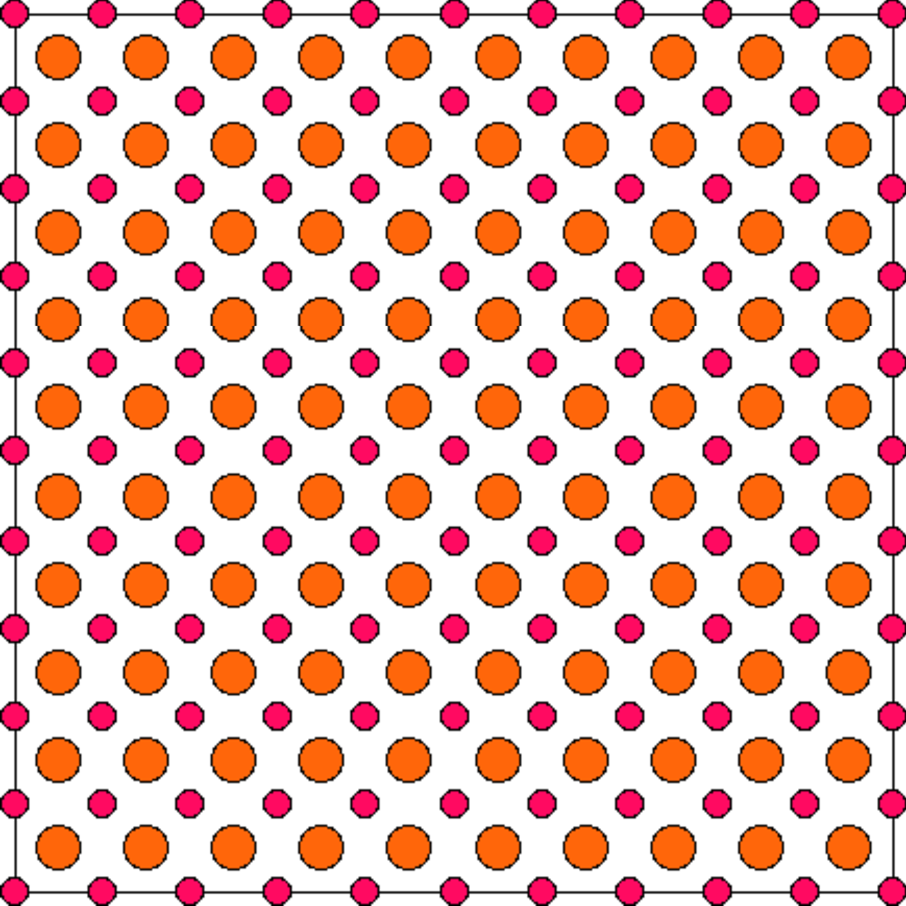
\includegraphics[width=0.30\textwidth]{2_Literature_Review/Fig/GaAs_100.pdf}};
            \draw [fill = black] (0.15, 0.15) rectangle (-0.15, -0.15);
            \draw [white] (0.1, 0.1) -- (-0.1, -0.1);
            \draw [white] (-0.1, 0.1) -- (0.1, -0.1);
        \end{tikzpicture}
    }
    \subcaptionbox{
        \hkl{1 1 0} facet.
        \label{subfig:GaAs_110}
    }{
        \tikzsetnextfilename{GaAs_110}
        \begin{tikzpicture}
            \node[inner sep=0pt] (image) at (0, 0) {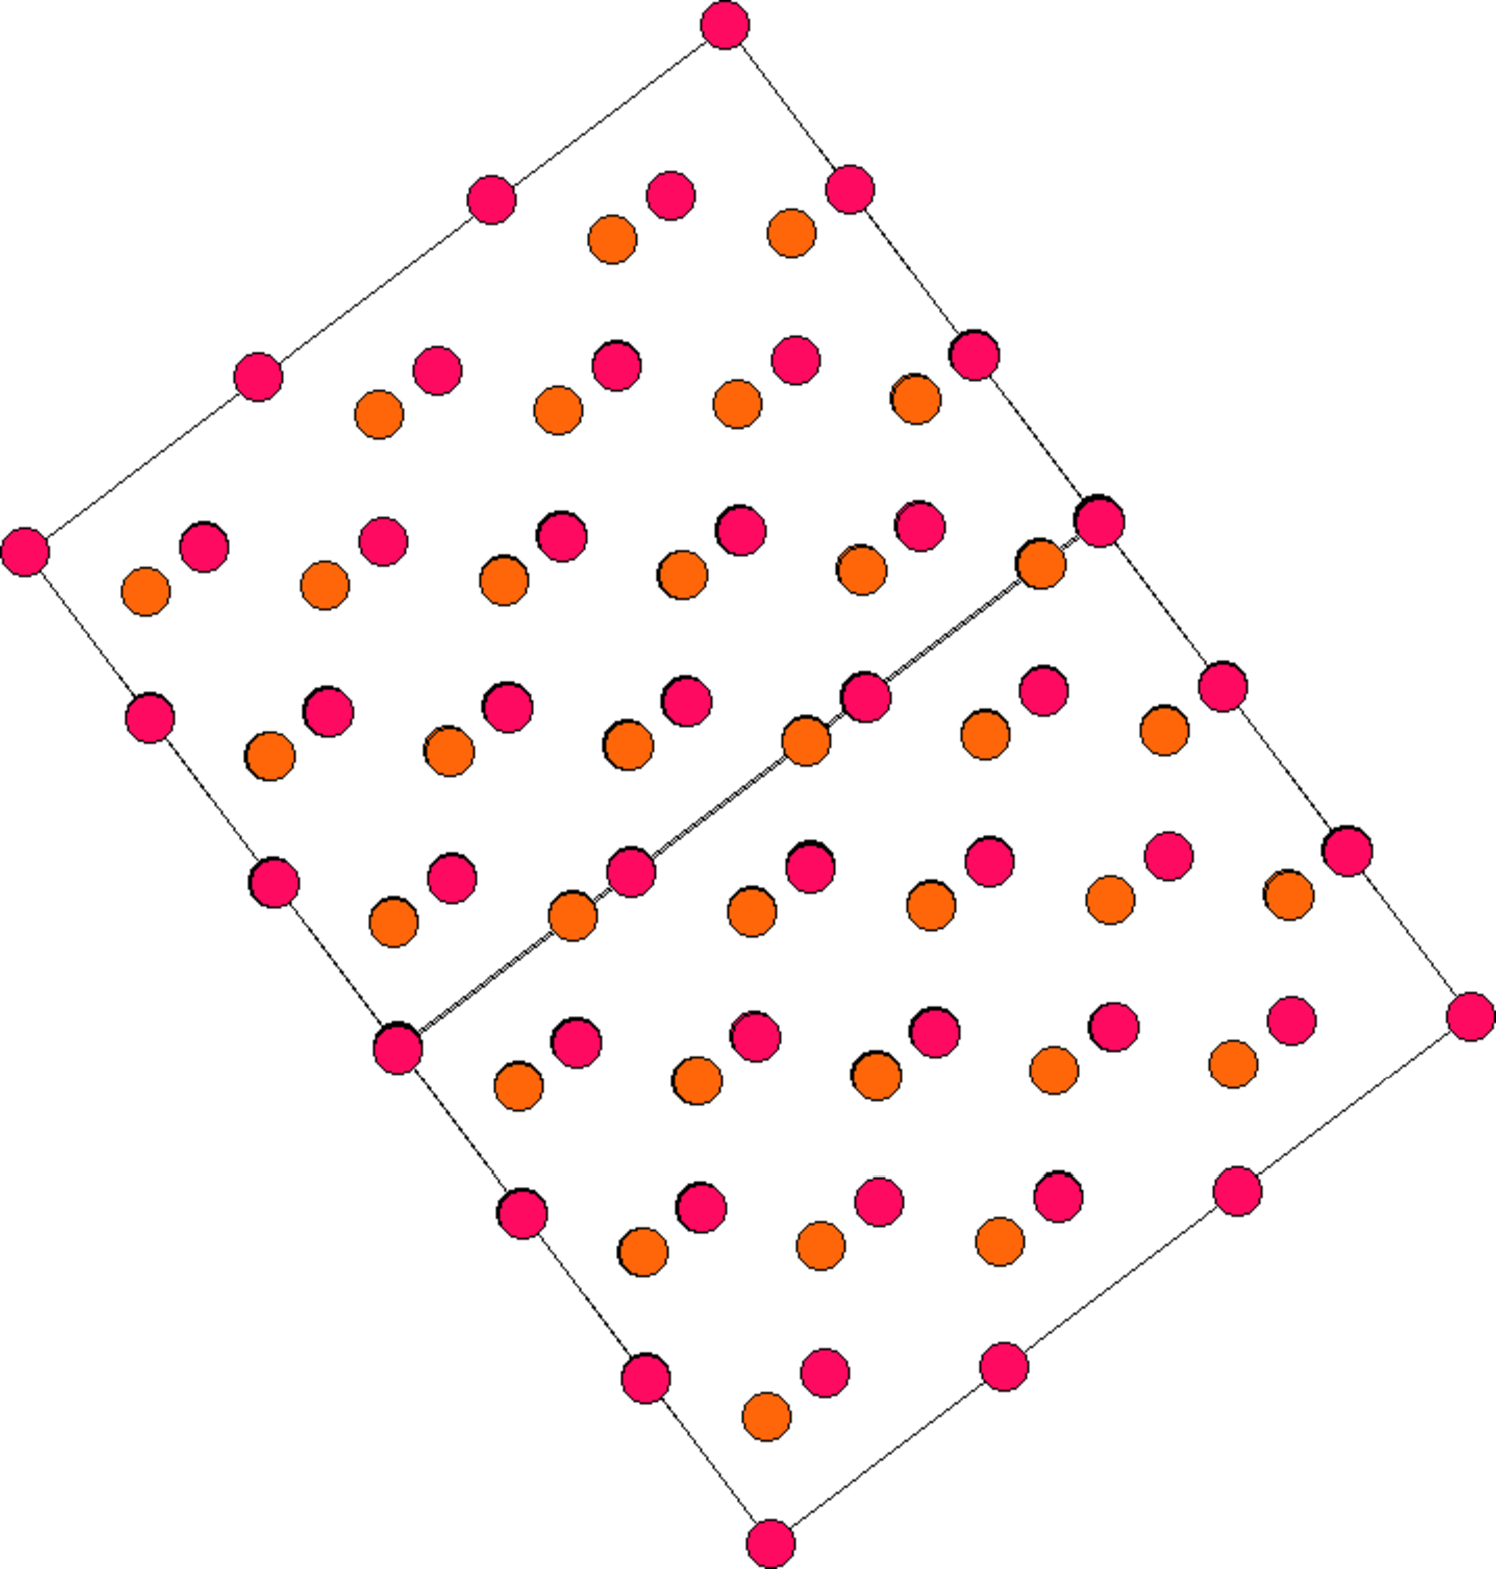
\includegraphics[width=0.30\textwidth]{2_Literature_Review/Fig/GaAs_110.pdf}};
            \begin{scope}[yshift=-0.01]
                \draw (0, 0) -- ++ (37:2);
                \draw (0, 0) -- ++ (37:-2);
                \draw (34:1.9) -- ++ (37:-0.3) -- ++ (-53:0.1) -- cycle;
                \draw (40:1.9) -- ++ (37:-0.3) -- ++ (127:0.1) -- cycle;
            \end{scope}
        \end{tikzpicture}
    }
    \subcaptionbox{
        \hkl{1 1 1}\(_B\) facet.
        \label{subfig:GaAs_111}
    }{
        \tikzsetnextfilename{GaAs_111}
        \begin{tikzpicture}
            \node[inner sep=0pt] (image) at (0, 0) {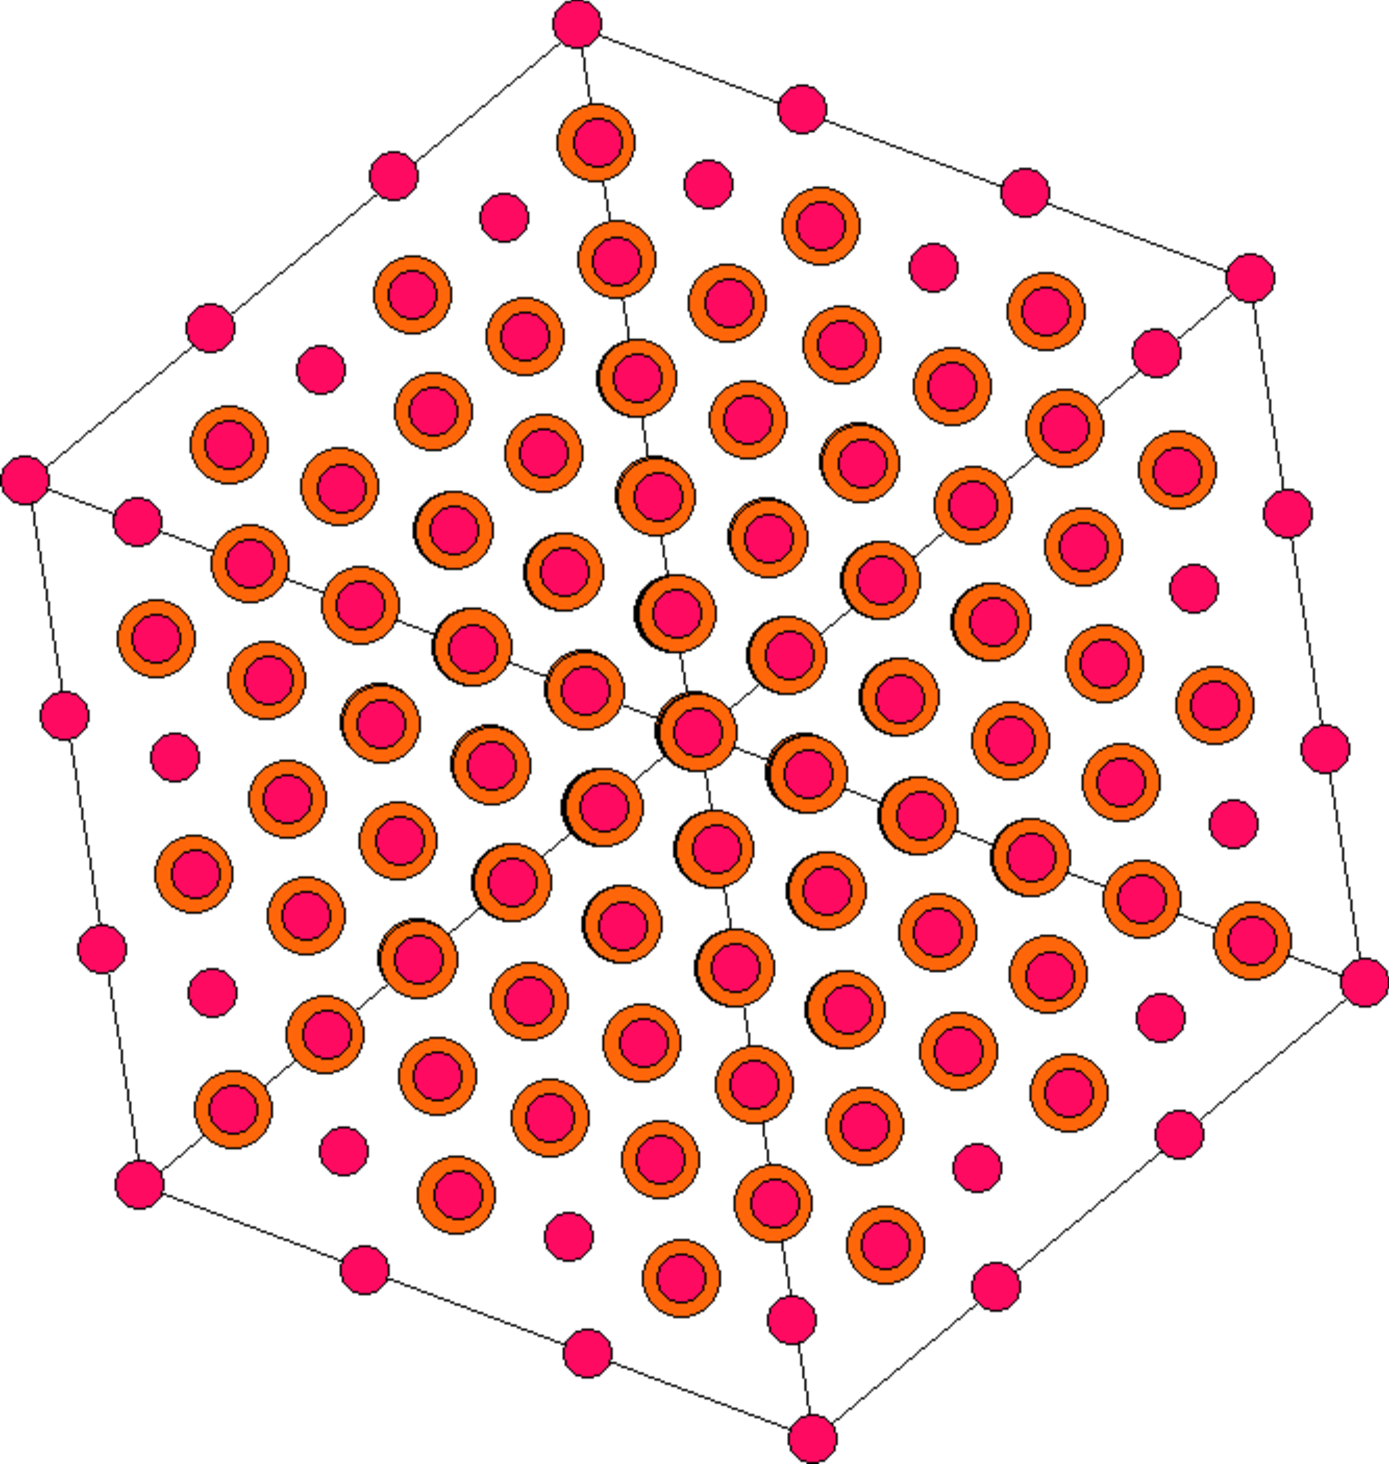
\includegraphics[width=0.30\textwidth]{2_Literature_Review/Fig/GaAs_111.pdf}};
            \draw [fill = black] (0.17, 0) -- ++ (-150:0.3) -- ++ (90:0.3) -- cycle;
            \draw [white] (0, 0) -- ++ (-120:0.1);
            \draw [white] (0, 0) -- ++ (0:0.1);
            \draw [white] (0, 0) -- ++ (120:0.1);
        \end{tikzpicture}
    }
    \caption[Low-index facets in the F\(\bar{4}\)3m \acs{gaas} crystal.]{2D projections of the low-index facets in the F\(\bar{4}\)3m \acs{gaas} crystal with the basic symmetry elements highlighted. \Acl{ga} is represented in orange and \acs{as} in pink; atomic radii are not to scale. \subref{subfig:GaAs_100} shows the 2D projection of the lattice along the \hkl{0 0 1} direction, which coincides with the four-fold axis. \subref{subfig:GaAs_110} shows the 2D projection along the \hkl{1 1 0} direction, contained in the mirror plane. \subref{subfig:GaAs_111} shows the 2D projection along the \hkl{1 1 1} direction, coinciding with the three-fold axis.}
    \label{fig:ZB_low_index_facets}
\end{figure}

III-V semiconductors are compound semiconductors formed by the stoichiometric combination of elements from the III group (third group, or group thirteen in the modern nomenclature) and the V group (fifth group, or group fifteen) of the periodic table. In their simplest form, they are binary, consisting of one III group and one V group element, with some examples being \acs{inp} and \acs{gaas}. Ternary and quaternary III-V materials such as \ce{In1_-_xGa_xAs} or \ce{In1_-_xGa_xAs1_-_yP_y} contain three or four different elements, respectively. 

Crystallographically, III-V materials are available at room temperature in crystals with the symmetries of space group number \num{216} (F\(\bar{4}\)3m, or zincblende-like) or \num{186} (P6\(_3\)mc, or wurtzite-like) and are easily affected by polytypism when grown. Space group \num{216} is that of a cubic face-centred crystal, while space group \num{186} describes a hexagonal crystal. These two structures are closely related, as the addition of a two-fold axis alongside the three-fold axis of space group \num{216} results in a phase change to space group \num{186}, transforming the affected \hkl<1 1 1> direction in the zincblende phase to the \hkl<0 0 0 1> direction in the wurtzite phase. \hkl{1 1 1} facets can also be described according to which half of the AB stoichiometry of the III-V material is exposed. For example, in Figure~\ref{subfig:GaAs_111} the top layer is entirely composed of V group atoms. This facet is called a \hkl{1 1 1}\(_B\) facet, while a \hkl{1 1 1}\(_A\) facet has III group atoms exposed.

Figure~\ref{fig:ZB_low_index_facets} shows the 2D projections of a \acs{gaas} F\(\bar{4}\)3m crystal along the low-index directions. These projections are useful for interpreting atomic-resolution microscopy images of III-V semiconductors. These computer-generated projections were created using CrystalKit, a dedicated software. They also highlight the main symmetry elements of the zincblende space group. The 2D projection in Figure~\ref{subfig:GaAs_100} shows how a \hkl{0 0 1} facet appears in the microscope. The symmetry element controlling its motif is a four-fold axis perpendicular to the projection plane. Similarly, Figure~\ref{subfig:GaAs_110} shows how a \hkl{1 1 0} facet appears in the microscope and the mirror plane dictating its symmetry. Finally, Figure~\ref{subfig:GaAs_111} shows the lattice projected along the \hkl<1 1 1> direction. The symmetry of this projection is compatible with a three-fold axis coinciding with the \hkl<1 1 1> vector.

\begin{figure}
    \centering
    \subcaptionbox{
        \hkl[0 0 1] corresponding to the z-axis.
        \label{subfig:100_symmetry}
    }{
        \tikzsetnextfilename{100_symmetry}
        \begin{tikzpicture}[isometric]
            \draw [fill=cb1_orange] (0.5, 0.5, 1.5) -- (-0.5, 0.5, 1.5) -- (-0.5, -0.5, 1.5) -- (0.5, -0.5, 1.5) -- cycle;
            % \draw [fill=red] (0.5, 0.5, -1.5) -- (-0.5, 0.5, -1.5) -- (-0.5, -0.5, -1.5) -- (0.5, -0.5, -1.5) -- cycle;
            \draw [fill=cb1_orange] (1.5, 0.5, 0.5) -- (1.5, -0.5, 0.5) -- (1.5, -0.5, -0.5) -- (1.5, 0.5, -0.5) -- cycle;
            % \draw [fill=green] (-1.5, 0.5, 0.5) -- (-1.5, -0.5, 0.5) -- (-1.5, -0.5, -0.5) -- (-1.5, 0.5, -0.5) -- cycle;
            \draw [fill=cb1_orange] (0.5, 1.5, 0.5) -- (-0.5, 1.5, 0.5) -- (-0.5, 1.5, -0.5) -- (0.5, 1.5, -0.5) -- cycle;
            % \draw [fill=blue] (0.5, -1.5, 0.5) -- (-0.5, -1.5, 0.5) -- (-0.5, -1.5, -0.5) -- (0.5, -1.5, -0.5) -- cycle;
            \draw [fill=cb1_light_blue] (1.5, 0.5, 0.5) -- (1.5, -0.5, 0.5)-- (0.5, -0.5, 1.5) -- (0.5, 0.5, 1.5)  -- cycle;
            \draw [fill=cb1_purple] (0.5, 0.5, 1.5)  -- (1.5, 0.5, 0.5) -- (0.5, 1.5, 0.5) -- cycle;
            \draw [fill=cb1_purple] (0.5, -0.5, 1.5)  -- (1.5, -0.5, 0.5) -- (0.5, -1.5, 0.5) -- cycle;
            \draw [fill=cb1_light_blue] (0.5, 0.5, 1.5) -- (-0.5, 0.5, 1.5) -- (-0.5, 1.5, 0.5) -- (0.5, 1.5, 0.5) -- cycle;
            \draw [fill=cb1_light_blue] (0.5, 1.5, -0.5) -- (0.5, 1.5, 0.5) -- (1.5, 0.5, 0.5) -- (1.5, 0.5, -0.5) -- cycle;
            \draw [fill=cb1_purple] (0.5, 0.5, -1.5) -- (0.5, 1.5, -0.5) -- (1.5, 0.5, -0.5) -- cycle;
            \draw [fill=cb1_purple] (-0.5, 0.5, 1.5) -- (-0.5, 1.5, 0.5) -- (-1.5, 0.5, 0.5) -- cycle;
            \draw [-stealth] (0,0,1.5) -- ++ (0,0,1) node [anchor=east] {\hkl[1 0 0]};
            \draw [-stealth] (0,1.5,0) -- ++ (0,1,0) node [anchor=south] {\hkl[0 0 1]};
            \draw [-stealth] (1.5,0,0) -- ++ (1,0,0) node [anchor=west] {\hkl[0 1 0]};
        \end{tikzpicture}
    }
    \subcaptionbox{
        \hkl[1 1 0] corresponding to the z-axis.
        \label{subfig:110_symmetry}
    }{
        \tikzsetnextfilename{110_symmetry}
        \begin{tikzpicture}[isometric]
            \begin{scope}[rotate around x=45]
                \draw [fill=cb1_orange] (0.5, 0.5, 1.5) -- (-0.5, 0.5, 1.5) -- (-0.5, -0.5, 1.5) -- (0.5, -0.5, 1.5) -- cycle;
                \draw [fill=red] (0.5, 0.5, -1.5) -- (-0.5, 0.5, -1.5) -- (-0.5, -0.5, -1.5) -- (0.5, -0.5, -1.5) -- cycle;
                \draw [fill=cb1_orange] (1.5, 0.5, 0.5) -- (1.5, -0.5, 0.5) -- (1.5, -0.5, -0.5) -- (1.5, 0.5, -0.5) -- cycle;
                % \draw [fill=green] (-1.5, 0.5, 0.5) -- (-1.5, -0.5, 0.5) -- (-1.5, -0.5, -0.5) -- (-1.5, 0.5, -0.5) -- cycle;
                \draw [fill=cb1_orange] (0.5, 1.5, 0.5) -- (-0.5, 1.5, 0.5) -- (-0.5, 1.5, -0.5) -- (0.5, 1.5, -0.5) -- cycle;
                % \draw [fill=blue] (0.5, -1.5, 0.5) -- (-0.5, -1.5, 0.5) -- (-0.5, -1.5, -0.5) -- (0.5, -1.5, -0.5) -- cycle;
                \draw [fill=cb1_light_blue] (1.5, 0.5, 0.5) -- (1.5, -0.5, 0.5) -- (0.5, -0.5, 1.5) -- (0.5, 0.5, 1.5)  -- cycle;
                \draw [fill=cb1_purple] (0.5, 0.5, 1.5)  -- (1.5, 0.5, 0.5) -- (0.5, 1.5, 0.5) -- cycle;
                % \draw [fill=cb1_purple] (0.5, -0.5, 1.5)  -- (1.5, -0.5, 0.5) -- (0.5, -1.5, 0.5) -- cycle;
                \draw [fill=cb1_light_blue] (0.5, 0.5, 1.5) -- (-0.5, 0.5, 1.5) -- (-0.5, 1.5, 0.5) -- (0.5, 1.5, 0.5) -- cycle;
                \draw [fill=cb1_light_blue] (0.5, 1.5, -0.5) -- (0.5, 1.5, 0.5) -- (1.5, 0.5, 0.5) -- (1.5, 0.5, -0.5) -- cycle;
                \draw [fill=cb1_purple] (0.5, 0.5, -1.5) -- (0.5, 1.5, -0.5) -- (1.5, 0.5, -0.5) -- cycle;
                \draw [fill=cb1_purple] (-0.5, 0.5, 1.5) -- (-0.5, 1.5, 0.5) -- (-1.5, 0.5, 0.5) -- cycle;
                \draw [fill=cb1_light_blue] (-0.5, 0.5, -1.5) -- (-0.5, 1.5, -0.5) -- (0.5, 1.5, -0.5) -- (0.5, 0.5, -1.5) -- cycle;
                \draw [fill=cb1_light_blue] (1.5, -0.5, -0.5) -- (1.5, 0.5, -0.5) -- (0.5, 0.5, -1.5) -- (0.5, -0.5, -1.5) -- cycle;
                \draw [fill=cb1_light_blue] (-1.5, 0.5, -0.5) -- (-1.5, 0.5, 0.5) -- (-0.5, 1.5, 0.5) -- (-0.5, 1.5, -0.5) -- cycle;
                \draw [fill=cb1_purple] (-0.5, 0.5, -1.5) -- (-1.5, 0.5, -0.5) -- (-0.5, 1.5, -0.5) -- cycle;
                \draw [-stealth] (0,0,-1.5) -- ++ (0,0,-1) node [anchor=south] {\hkl[1 0 0]};
                \draw [-stealth] (0,1.5,0) -- ++ (0,1,0) node [anchor=east] {\hkl[0 1 0]};
                \draw [-stealth] (1.5,0,0) -- ++ (1,0,0) node [anchor=west] {\hkl[0 0 1]};
            \end{scope}
        \end{tikzpicture}
    }
    \caption[Low index facet orientation in the F\(\bar{4}\)3m space group.]{Low index facet orientation in the F\(\bar{4}\)3m space group. The \hkl{0 0 1}, \hkl{1 1 0}, and \hkl{1 1 1} facets are color-coded in orange, light blue, and purple, respectively. The two orientations shown in this Figure are with the vertical z-axis coinciding with the \hkl[0 0 1] and \hkl[1 1 0] directions in \subref{subfig:100_symmetry} and \subref{subfig:110_symmetry}, respectively.}
    \label{fig:facet_relations}
\end{figure}

Although the orientation of the low index facets with respect to each other is difficult to properly convey in a 2D projection, Figure~\ref{fig:facet_relations} shows how the three different facets, \hkl{0 0 1} in orange, \hkl{1 1 0} in light blue, and \hkl{1 1 1} in purple, are orientated in a cubic crystal. The shapes of the polygons that make up the figure also give a hint as to what kind of symmetry element is present in each facet. Figure~\ref{subfig:100_symmetry} can also be used to understand the relationship between different planes in the cubic \acl{si} crystal of the \hkl(0 0 1) \acf{soi} device layer used as growth substrate in Chapter~\ref{chap:growth}. Similarly, Figure~\ref{subfig:110_symmetry} illustrates the symmetry of the \hkl(1 1 0) \acs{soi} device layer used in Chapters~\ref{chap:properties} and \ref{chap:yield_analysis}.

\begin{figure}
    \centering
    \tikzsetnextfilename{GaAs_rtp}
    \begin{tikzpicture}
        \node[inner sep=0pt] (image) at (0, 0) {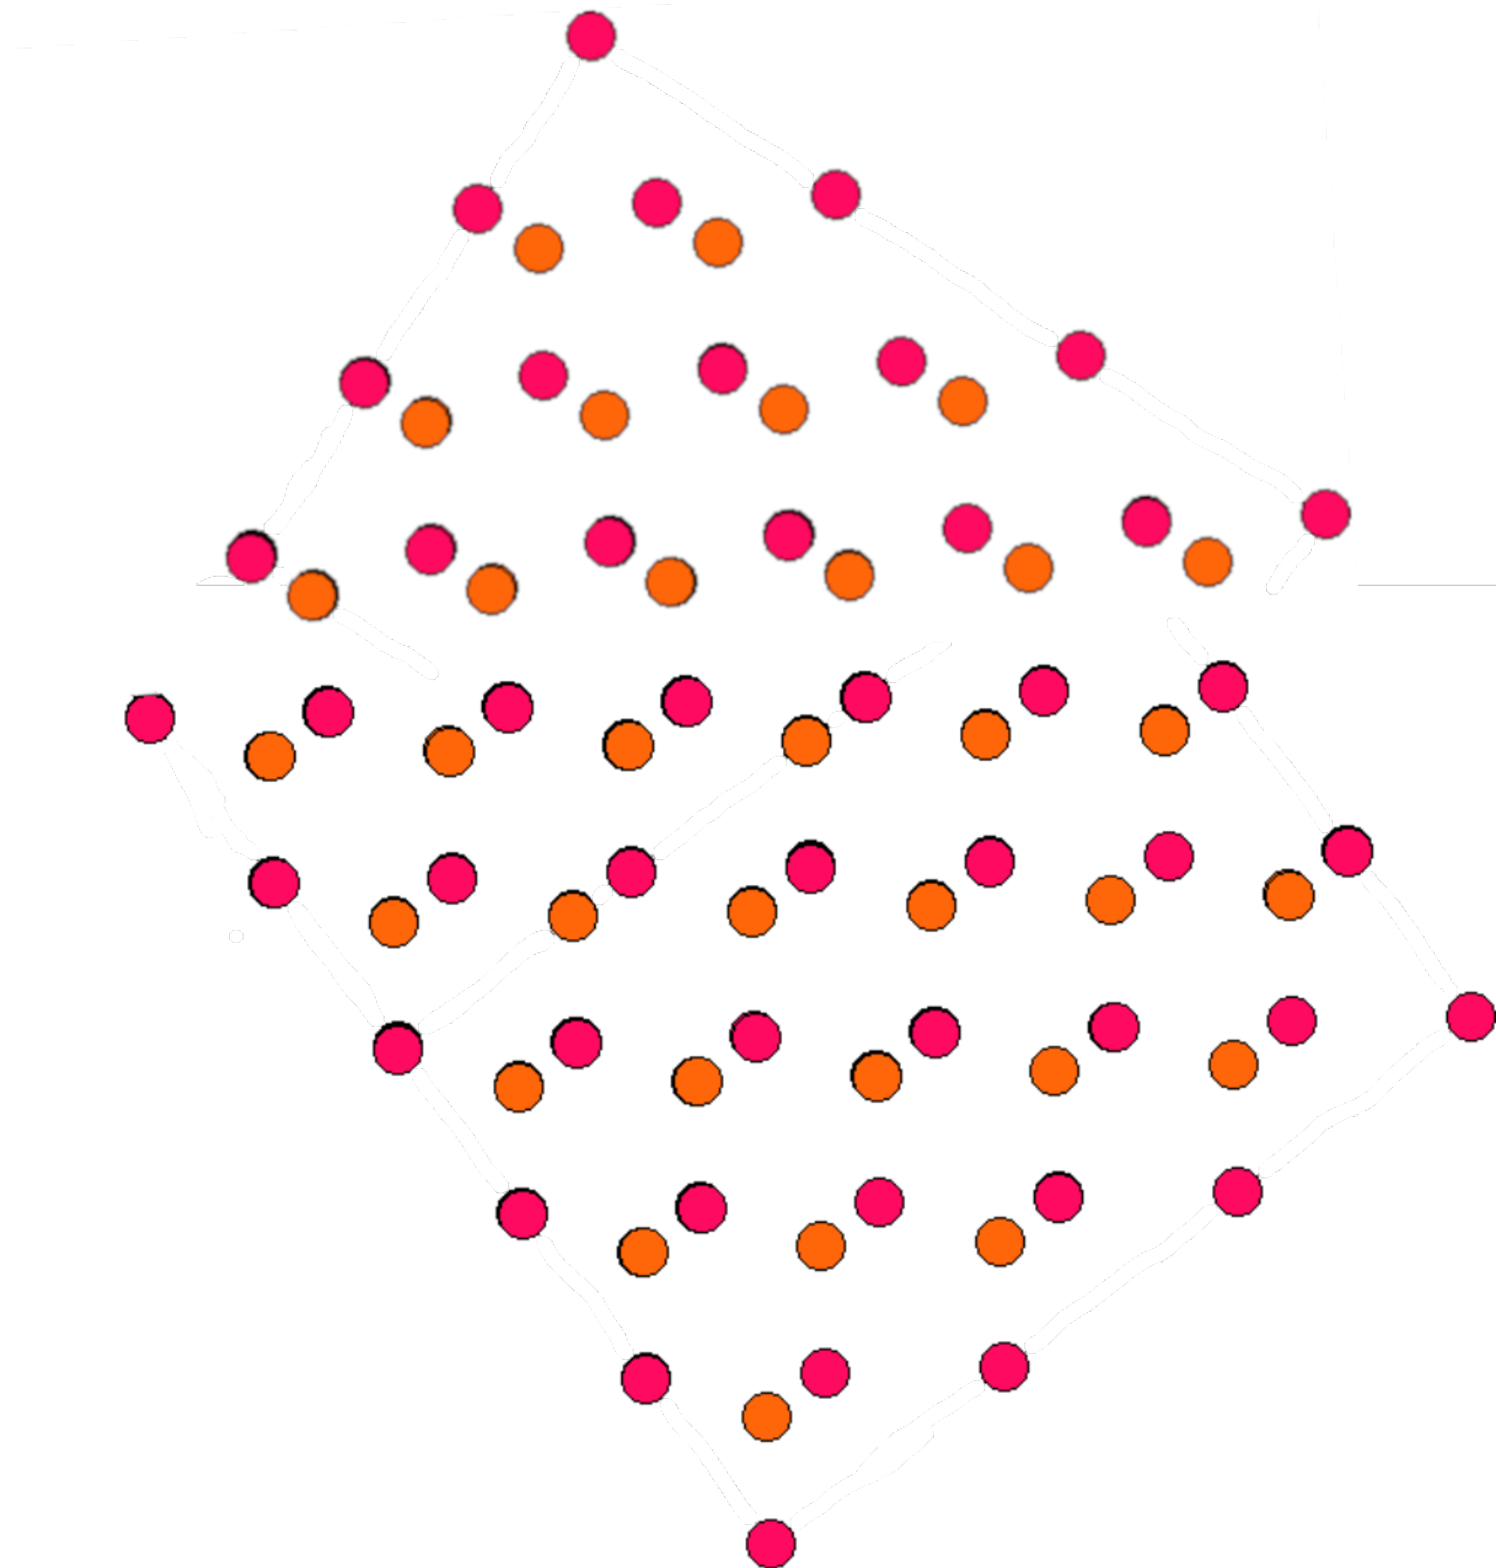
\includegraphics[width=0.3\textwidth]{2_Literature_Review/Fig/GaAs_rtp.pdf}};
        \draw [dashed] (-2.5,0.4) -- ++ (5,0.15) node [anchor = west] {RTP};
    \end{tikzpicture}
    \caption[Drawing of a \hkl{1 1 1} \acl{rtp} in a F\(\bar{4}\)3m crystal.]{Drawing of a \acf{rtp}, highlighted by a dashed line, corresponding to a \hkl{1 1 1} plane in a \acs{gaas} F\(\bar{4}\)3m crystal.}
    \label{fig:GaAs_rtp}
\end{figure}

Figure~\ref{fig:GaAs_rtp} shows a drawing of a \acf{rtp} corresponding to a \hkl{1 1 1} plane in a \acs{gaas} F\(\bar{4}\)3m crystal. Formation of this type of 2D defect is common in the growth of III-V crystals \cite{Borg2017} and its density is very sensitive to changes in the growth environment \cite{Algra2008, Chi2013} due to its low formation energy. From a lattice symmetry point of view, the \acs{rtp} is formed by adding a two-fold rotation axis to the \hkl{1 1 1} direction of the crystal. The two atomic bilayers adjacent to the \acs{rtp} can be considered a thin slice of wurtzite \cite{Glas2007, Vedel2022}.

Both atomic species and lattice symmetry affect the electronic properties of crystals. Bloch functions are the eigenfunctions of the Hamiltonian that describe a particle in a periodic potential \cite{Dirl2005}, and pose the basis for understanding the behaviour of electrons in crystals. They are also periodic functions, and in reciprocal space they are used to describe the electronic band structure, resulting in plots such as those in Figure~\ref{fig:band_structure}. The band structures in this figure were calculated, using \acf{dft}, and then plotted by Christian Dam Vedel. Energy is on the vertical axis, with its origin at the Fermi energy, which is the energetic midpoint between the last occupied state and the first unoccupied state, at \qty{0}{\kelvin} (thermal zero). The horizontal axis shows wavevectors along certain high-symmetry directions in the unit cell of the reciprocal lattice: the Brillouin zone \cite{Setyawan2010}. The energy of each of the states along the one-dimensional paths that link these points is then plotted. Therefore, in Figure~\ref{fig:band_structure}, the states below the Fermi energy are part of the valence band and those above it are part of the conduction band. 

\begin{figure}
    \centering
    \subcaptionbox{
        Band structure of F\(\bar{4}\)3m \acs{inp}.
        \label{subfig:ZB_bands_InP}
    }{
        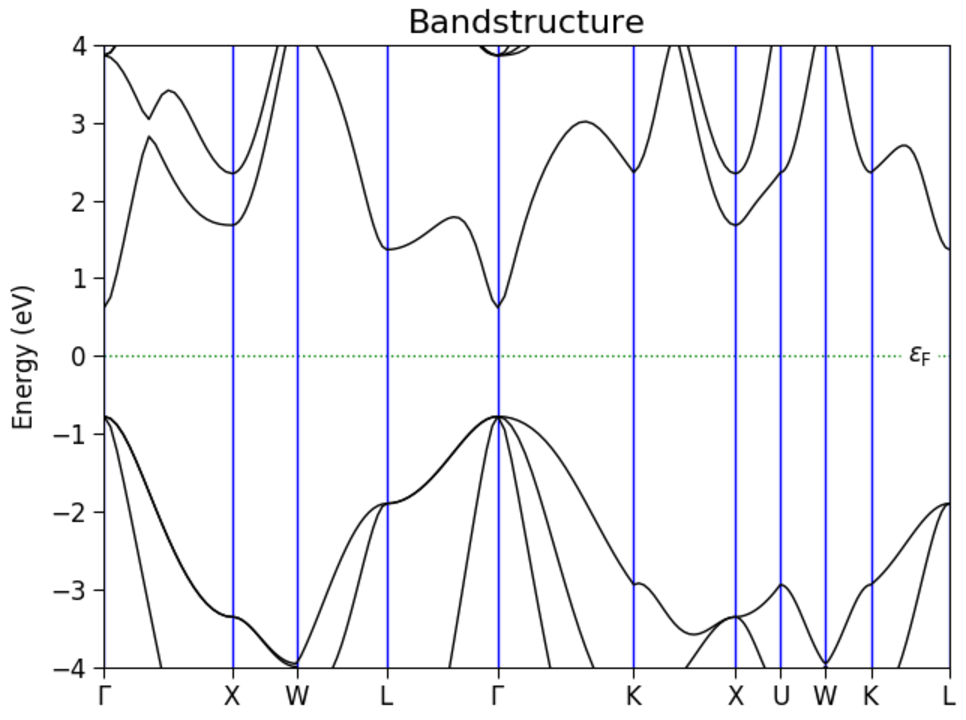
\includegraphics[width=0.48\textwidth]{2_Literature_Review/Fig/Zincblende_bandstructure_InP.pdf}
    }
    \subcaptionbox{
        Band structure of P6\(_3\)mc \acs{inp}.
        \label{subfig:WZ_bands_InP}
    }{
        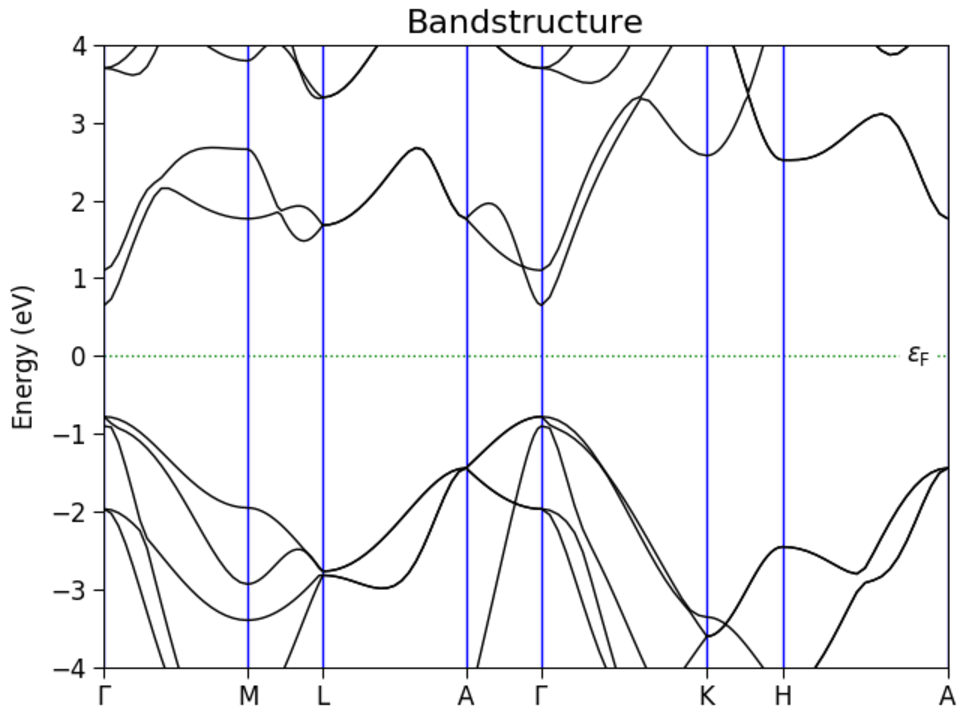
\includegraphics[width=0.48\textwidth]{2_Literature_Review/Fig/Wurtzite_bandstructure_InP.pdf}
    }
    \subcaptionbox{
        Band structure of Fd\(\bar{3}\)m \acs{si}.
        \label{subfig:Si_bands}
    }{
        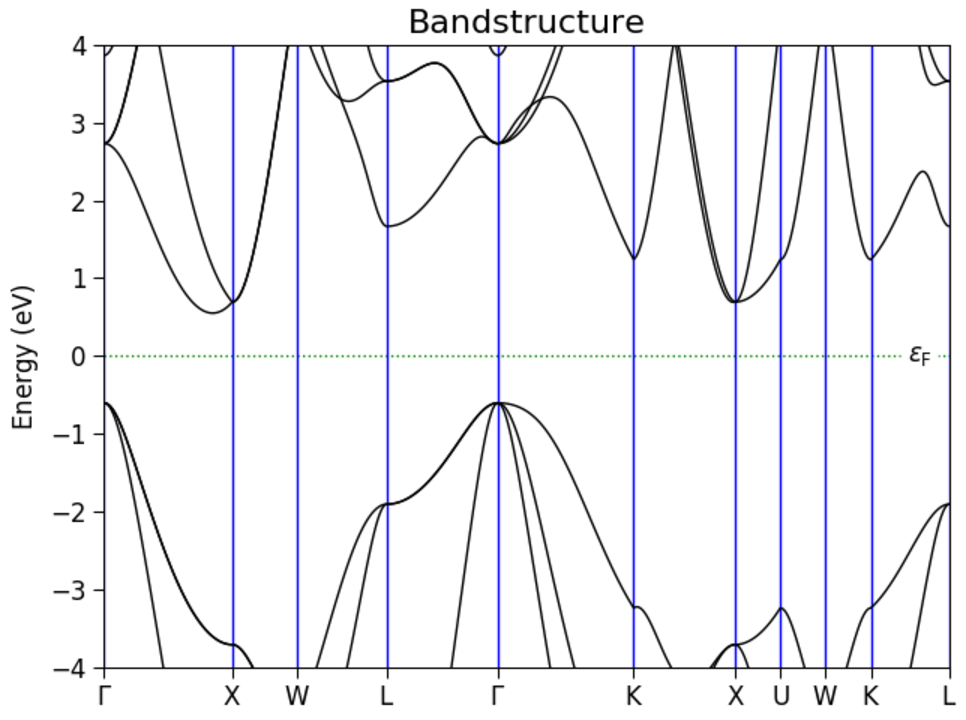
\includegraphics[width=0.48\textwidth]{2_Literature_Review/Fig/Silicon_bandstructure.pdf}
    }
    \caption[Band structures of \acl{si}, and \acs{inp} in its cubic and hexagonal phases.]{Band structures of \acl{si}, and \acs{inp} in its cubic and hexagonal phases, calculated with \acs{dft}. \subref{subfig:ZB_bands_InP} and \subref{subfig:WZ_bands_InP} show the band structures of zincblende and wurtzite \acs{inp}. The Fermi energy (\(\epsilon_F\)) defines the origin of the ordinate and is marked by a dotted line.  \subref{subfig:Si_bands} shows the band structure of Fd\(\bar{3}\)m \acs{si}. Images courtesy of Christian Dam Vedel.}
    \label{fig:band_structure}
\end{figure}

The $\Gamma$ point is the centre of the Brillouin zone and is very important for understanding photon-driven electronic transitions between bands. A material with the minimum of the conduction band and the maximum of the valence band at the $\Gamma$ point is said to have a direct band gap. Conversely, a material that has a band structure with the minimum of the conduction band at a wavevector that is different from the wavevector of the maximum of the valence band is said to have an indirect band gap. Due to momentum conservation rules, a single photon can only cause so-called centrezone transitions, which are transitions between states at the $\Gamma$ point. Interband transitions outside of the centrezone require a third particle, usually a phonon, to mediate the transition, changing the type of interaction from two-particle to three-particle; which has a lower probability of occurring. Similarly, the radiative relaxation pathway is prevalent in direct band-gap semiconductors, while non-radiative relaxation paths are prevalent in indirect band-gap semiconductors.

Therefore, the band gap type greatly affects a semiconductor's light-emitting and -absorbing properties. III-V semiconductors have direct band gaps, as exemplified by those of the zincblende and wurtzite phases of  \acl{inp} shown in Figures~\ref{subfig:ZB_bands_InP} and \ref{subfig:WZ_bands_InP}, and are highly efficient light emitters and absorbers as a consequence. On the contrary, \acl{si} has an indirect bandgap, as shown in Figure~\ref{subfig:Si_bands}, making it an ill-suited material for light emission and absorption.

Tuning a semiconductor's band gap is key to the control of its absorption and emission wavelengths. Although binary III-Vs provide fixed starting points in both band gap and lattice constant, ternary and quaternary III-V compounds allow high-precision tuning of both properties \cite{Ning2017}. For example, the materials chosen by the \acs{design} consortium were \acs{inp} and \ce{In0_.53Ga0_.47As}, because they are lattice-matched and therefore a lower density of defects is expected at their interface \cite{Pearsall1980, Sugii1983, Wagner1970} and because \acs{ingaas} emits in the telecom range \cite{Scherrer2021, Seravalli2020}.

\section{\texorpdfstring{III-V-on-\acs{si} integration routes}{III-V-on-Si integration routes}}
Various III-V synthesis methods are available \cite{Kuech2016}: the following is an overview of epitaxial growth methods focussing on the integration routes of III-V semiconductors on \acl{si}, which can be divided into two broad categories: transfer and monolithic integration.

\subsection{Transfer integration}

Transfer integration refers to the indirect integration of III-V material grown on a different lattice-matched substrate on a \acl{si} wafer. 

The main advantage of these techniques is the absence of lattice mismatch as a source of defects during epitaxial growth. Furthermore, it allows the selection of the best-performing structures to be transferred onto the \acl{si} substrate \cite{Zadeh2016, Wang2017}. Transfer integration does not have to compromise on the growth parameters or material systems to achieve \acs{cmos} compatibility (except for bonding temperature). Together, the various methods that fall under this definition form a mature technology well established in industry \cite{Han2022, Wang2017}, and, as a result, benefit from years of industrial optimisation.

This type of integration requires the growth of III-V in a separate fabrication line that must maintain the high precision and cleanliness standard of the main \acs{cmos} \acl{si} line, resulting in a large capital investment. Furthermore, most classic transfer steps can result in a material with a more irregular geometry (wafer bow, surface roughness after etching), or presenting transfer-related defects \cite{Jevtics2022}, or require an extra bonding layer \cite{Tang2019, Audet1997, Cheng2000, Sparks2001}, and do not allow nanometre precision in integration \cite{McPhillimy2020, Wang2017}. However, the most advanced techniques that bypass most of these quality issues are too slow to provide a competitive transfer time for large, densely integrated \qty{200}{\milli\metre} (or \qty{300}{\milli\metre}) production wafers \cite{McPhillimy2020, Wang2017}.

\subsection{Monolithic integration}

Monolithic integration refers to direct integration by epitaxial growth of III-V semiconductors on a \acl{si} substrate. 

It naturally provides advantages such as extremely high spatial precision and accuracy for small device integration on wafer-scale substrates, which can be achieved in a shorter time frame compared to its transfer analogues \cite{Wang2017, Wei2023}. It has the potential to be a more economical alternative to heterogeneous integration. If the growth process can be integrated with current \acs{cmos} processes, its implementation in a \acs{cmos} line would eliminate the need to have a dedicated III-V fabrication facility running in parallel with a \acl{si}-based plant, especially if the use of III-V electronics is envisioned at the same time as III-V photonics \cite{Wang2017}. Thus, monolithic integration has the potential to reduce the capital cost required to integrate III-V photonics in different \acl{si}-based devices \cite{Wang2017, Tang2019}.

The main disadvantage of monolithic integration is the high lattice mismatch between \acl{si} and most III-V materials \cite{Kuech2016}. The effect of this mismatch in the material is the formation of strain-relaxing defects at the \acl{si} / III-V heterointerface \cite{Kunert2018, Shi2021}: these defects have a very detrimental effect on the performance and lifetime of a device \cite{Mahajan2000, Zenari2021}, and act as scattering or recombination centres \cite{Jeon2015}. The polar nature of III-V atomic bonds compared to nonpolar \acs{si}-\acs{si} bonds means that \acl{apb} (\acs{apb}s) can be created during growth on \acl{si} surfaces with monoatomic steps \cite{Kunert2018}, and most known surface treatments to eliminate nucleation sites for these defects occur in temperature ranges that are incompatible with the \acs{cmos} process \cite{Laracuente2003, Kunert2018, Miller2000}. Furthermore, materials that are known to grow at a higher temperature, such as III – nitrides \cite{Huang2017}, and substances that could have detrimental effects on the passivating of \acf{sio2} layers through their diffusion, such as gallium \cite{Miller2000} which readily diffuses in \acl{sio2} \cite{VanOmmen1987}, also pose temperature-related \acs{cmos} compatibility issues. Another key obstacle, especially related to the direct growth of micro- and nanostructures, is the stricter requirements for the reproducibility and reliability of the process.

There are many monolithic integration routes, and the most common categories are introduced in the following paragraphs.

\paragraph{Planar growth} Direct planar growth of III-Vs on \acl{si} is the simplest method of monolithic integration. It can be suitable for the growth of III-Vs with a lattice constant very close to that of \acl{si} or for the self-assembled nucleation of nanoparticles in a Stranski-Krastanov growth mode, which can pose the basis for quantum dot fabrication \cite{Shi2016, Reithmaier2016}. It, however, presents a few drawbacks related to the absence of a way to contain defects and the different material properties of the material stack \cite{Ravash2012}. It can lead to wafer bow or warp due to the mismatch of thermal coefficients between the various materials \cite{Miyoshi2016, Wang2017_2}, and materials with a high deviation from the \acl{si} lattice parameter can require strain management layers of \qty{1}{\micro\metre} or more to grow without defects \cite{Wang2017_2, Cantoro2012, Huang2022}.
\par
\paragraph{\Acf{sag}} \acs{sag} consists in the growth of III-V material from \acl{si} seeds located in openings in a horizontal mask of a material that does not promote nucleation, such as \acs{sio2}. These holes can be defined with different methods, from self-assembled masking to lithography. This type of growth results in nanostructures \cite{Cantoro2012} such as nanowires, both of a single material and in core-shell configurations with very high position control \cite{Tomioka2011}. Wafer bow and warp are not issues with \acs{sag}, since growth does not, unless promoted by accentuating lateral growth \cite{McKenzie2023}, end up forming a single material layer. However, in this technique, growth develops mainly in the vertical direction, and the presence of lateral growth can result in unwanted heterointerfaces.
\par
\paragraph{Droplet epitaxy} Droplet or \acf{vls} epitaxy consists in guiding the nucleation of III-V material by using a nano-droplet of a catalyst metal on the \acl{si} substrate. This technique also avoids wafer bow as it only results in the growth of nanowires \cite{Wagner1964}. Since \acs{vls} is dependent on the metallic droplet, the growth can be tuned to achieve high directionality and the incorporation of heterostructures with minimal or no unwanted side growth \cite{Harmand2018, Joyce2007}. This type of growth depends on the metal droplets and therefore on their self-assembled distribution on the substrate surface, which diminishes position control \cite{Joyce2007}. Similarly, the geometry of the resulting structures is limited to nanowires \cite{Wagner1964}, and the reservoir effect in the catalyst droplet complicates the control of composition in ternary and quaternary III-V materials \cite{Dubrovskii2017}. Nonetheless, this method allows for sophisticated growth studies such as in-situ TEM imaging \cite{Harmand2018, Maliakkal2020, Jacobsson2016}, leading to the possible refinement of growth recipes to the point where phase control can be achieved \cite{Algra2008, Joyce2007, Caroff2009}.
\par
\paragraph{\Acf{art}} \acs{art} refers to the confinement of defects to the seed region by sidewalls and other such barriers in a growth regimen mediated by a template. The basic idea is that, as most defects nucleate near the \acl{si} / III-V interface and then propagate in directions that are often not parallel to the growth axis, they can be trapped in the region of the material closest to the seed by sidewalls that constrict the III-V crystal so that it grows in a cavity with a high aspect ratio. 

\acs{sag}-\acs{art} has the mask selecting the seed areas increase in thickness to allow the trapping of defects. This technique also allows high position control of the III-V crystal, while accentuating control over the defects \cite{Han2016, Han2016_2}. However, typically \acs{sag}-\acs{art} employs large templates, which means that defects propagating in directions that lie in the plane of the side walls are not filtered by the \acs{art} mechanism \cite{Kunert2018}. Simultaneously, multiple nucleation points in large seed areas can result in coalescence-borne defects often not trapped by sidewalls \cite{Kunert2016}.
\par
\paragraph{\Acf{tase}} \acs{tase} can be seen as an evolution of the \acs{sag}-\acs{art} method as it also defines \acl{si} seeds surrounded by \acs{sio2} and uses templates with high aspect ratio to guide growth. The main differences with \acs{sag}-\acs{art} are the size and complexity of the templates and the focus on planar growth. \acs{tase} enables the growth of various vertical and horizontal nanostructures while maintaining extremely accurate geometry and position control \cite{Ritter2021, Tiwari2020, Schmid2015}. It also enables superior defect control, even compared with \acs{art}: far from the growth interface, defects can be effectively limited to twin planes \cite{Han2020}, which can also be eliminated in some cases \cite{Knoedler2017}. In certain geometries, it also enables phase control \cite{Staudinger2018}. 

On the other hand, it is the most complex method of those listed in terms of overall steps before III-V growth. Furthermore, since nanowires fill templates quickly, \acs{tase} can only grow core-shell structures in a microdisk format \cite{Tiwari2020} and not in nanowire format. Like other techniques which employ a mask to control selectivity, unwanted nucleation on the masks, called parasitic growth, which results in parasitic crystals, can occur \cite{Goswami2021}.
\par

\section{\texorpdfstring{State of \acl{tase}}{State of template assisted selective epitaxy}}

As shown in the previous section, \acs{tase} is one of the most advanced monolithic integration techniques; its implementation can be found in Section~\ref{chap:tase}. The flexibility of \acs{tase} is demonstrated by the different ways research groups have used it. 

\subsection{Selection of nanofabrication process}

A group at the University of California Santa Barbara used \acs{tase} to achieve high facet control in the homoepitaxial growth of III-V semiconductors \cite{Brunelli2019, Goswami2020, Goswami2021}. Their growth approach mainly focusses on homoepitaxy of III-Vs on III-V substrates \cite{Brunelli2019, Goswami2020, Goswami2021}, which are more expensive compared to \acs{soi}. While growth dynamic studies from this group highlighting the role of low temperature and high V/III precursor ratios were instrumental in informing the growth parameters used in this thesis, a process based on \acs{soi} wafer was needed, as the growth findings of this project have the objective to further enable co-planar integration of active III-V components with \acs{si} waveguides.

The group at the University of Hong Kong focussed on deposition in large templates \cite{Han2020, Yan2021}. Sometimes the name \acf{lart} is used to highlight the use of large templates to create in-plane structures inside templates \cite{Han2020_2}. This method increases the risk of multiple nucleations and limits the defect-trapping effect in the in-plane direction \cite{Han2020, Yan2021, Huang2024}. As the \acs{lart} emitter fabrication methods used in the process adopted by this group are based on the etching of III-V \acs{lart} platelets \cite{Han2020_2, Huang2024}, the resulting devices are located far from waveguides. Furthermore, the use of etching in the fabrication process further complicates optimisation at the wafer scale, as both the growth and following etching parameters need to be tuned in order to create working devices.

The Hong Kong University and \acs{ibm} Research Europe - Zurich groups have been developing template-based methods to fully integrate planar \acs{pic}s on a \acs{soi} platform \cite{Mauthe2020}. This means a circuit made up of emitters, waveguides, and detectors. With the \acs{tase} method used in the Zurich group, \acl{si} waveguides can be defined in the same lithography step as emitting and absorbing structures, allowing for high design accuracy \cite{Wen2022}. Emitters can be integrated in the form of microdisks \cite{Tiwari2020, Tiwari2021}. \Acs{tase} microdisk devices, while demonstrating good performance, with evidence of lasing \cite{Tiwari2020}, suffer from the lower amount of gain material available with \acs{tase} compared with \acs{lart} \cite{Huang2024}. Alternatively, modulators can be made with \acs{tase} \cite{Scherrer2022, Scherrer2024} to substitute a dedicated emitter with the modulation of an existing light beam. Detectors can be made out of III-V \textit{p}-\textit{i}-\textit{n} structures in nanowires and have demonstrated high performance \cite{Mauthe2020, Wen2022}. The advantage of the \acs{tase} process employed in the Zurich group is that it allows for close coupling with co-planar \acs{si} waveguides, while avoiding the complications stemming from large seed areas. The growth study in this thesis supports the control of heterointerface in nanowire devices and, more specifically, the integration of quantum wells in \texttt{i} regions of \textit{p}-\textit{i}-\textit{n} structures. Nanowire \textit{p}-\textit{i}-\textit{n} detectors fabricated at \acs{ibm} Research Europe - Zurich have shown similar performance as bulkier \textit{p}-\textit{i}-\textit{n} detectors from the University of Hong Kong \cite{Mauthe2020, Wen2022, Xue2021}. Therefore, considering the existing know-how in Zurich, where the experimental part of my PhD took place, the \acs{ibm} \acs{tase} process was used in this work.

\subsection{\texorpdfstring{State of \acs{tase} at the beginning of the project}{State of TASE at the beginning of the project}}

\begin{figure}
    \centering
    \tikzsetnextfilename{wen}
    \begin{tikzpicture}
        \node[inner sep=0pt] (image) at (0, 0) {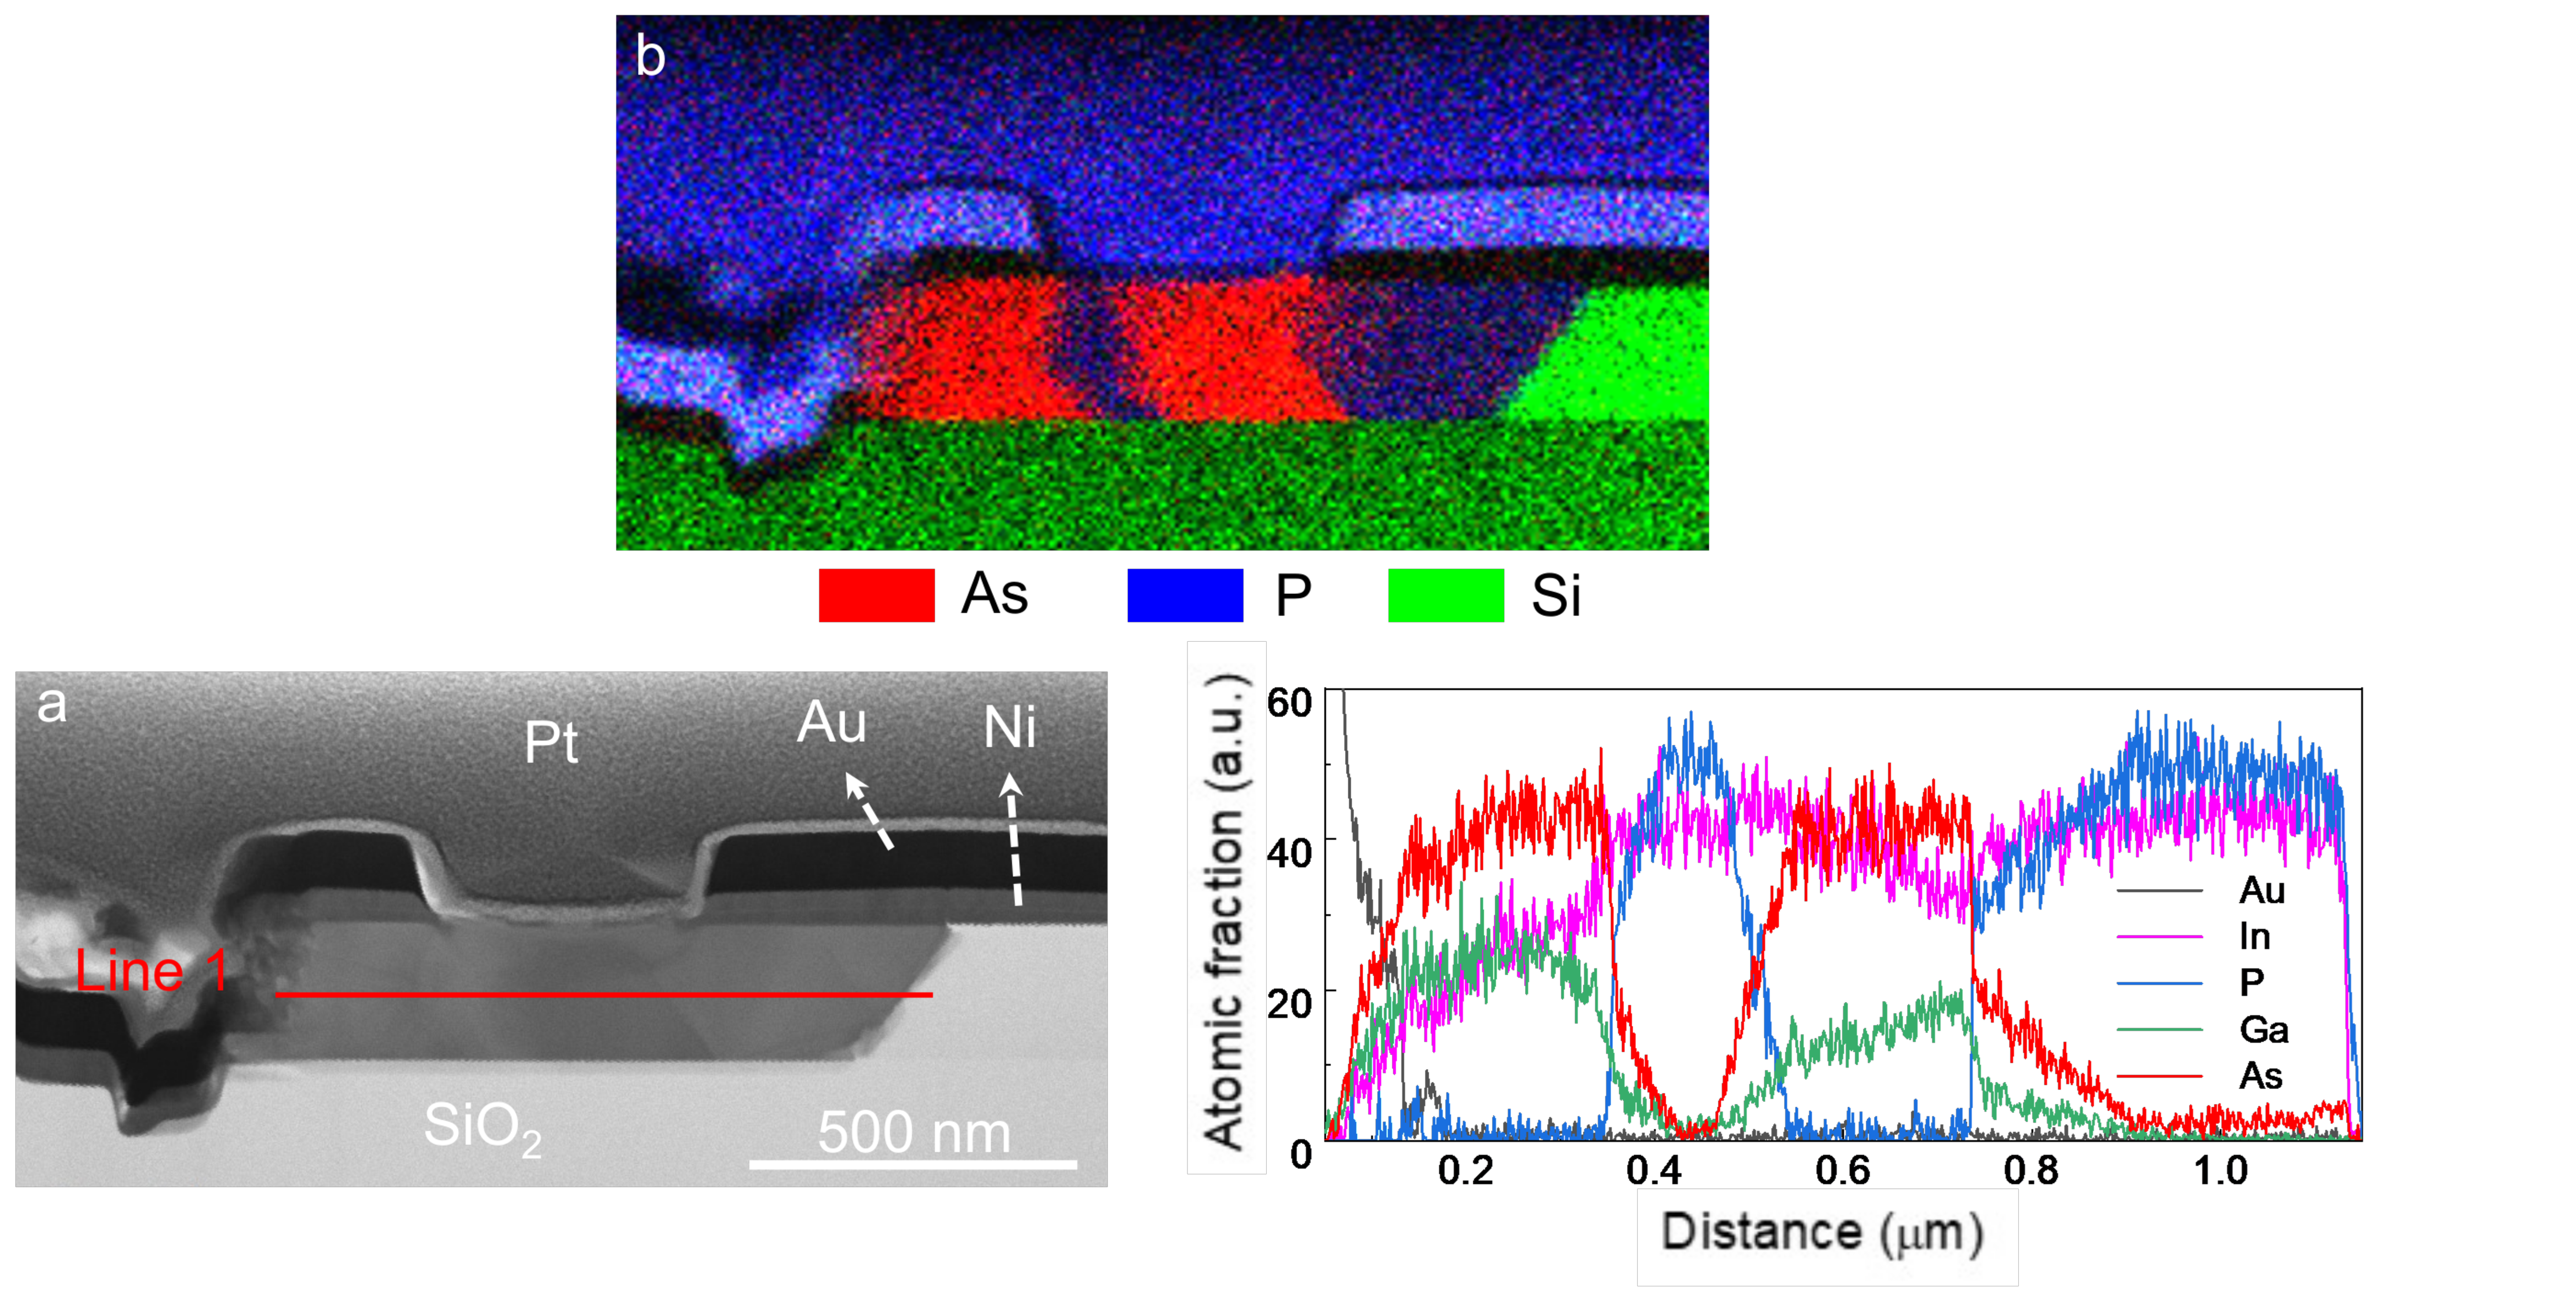
\includegraphics[width = \textwidth]{3_Growth/wen.pdf}};
        \node[fill=white] at (-7.6, -0.3) {(A)};
        \node[fill=white] at (-3.9, 3.7) {(B)};
        \node[fill=white] at (7.6, -0.3) {(C)};
    \end{tikzpicture}
    \caption[Structural and compositional analysis of a nanowire detector.]{Structural and compositional analysis of a nanowire detector carried out by Wen \textit{et al.} This Figure was adapted from the work of Wen et al \cite{Wen2022} under the terms of the CC BY 4.0 license \cite{CCBY40}.}
    \label{fig:wen}
\end{figure}

This project started with the backdrop of the device published by Wen et al. \cite{Wen2022}, shown in its structure in Figure~\ref{fig:wen}. The \acs{bf}-\acs{stem_m} image in Figure~\ref{fig:wen}(A) shows the morphology of the nanowire. A \hkl{1 1 1} \acf{si} facet on the right of the image served as the nucleation surface from which the heterostructures nanowire grew. The selection of this particular facet in \acs{tase} is not casual. The aim is to avoid monoatomic steps on the seed surface that can lead to the formation of \acs{apb}s \cite{Kunert2018}. Nickel-gold contacts are placed at the two \textit{p} and \textit{n} extremities of the doped III-V \textit{p}-\textit{i}-\textit{n} diode. These contact areas were defined specifically for the wire in question. 

Figure~\ref{fig:wen}(B) shows a composition map of the device created from \acf{eds} data. It can be seen that the internal structure of the nanowire contains multi-faceted heterointerfaces. This is exemplified by the first phosphide layer (counting from the \acl{si} seed on the right of the image towards the end of the wire on the left) which presents a bottom \hkl{1 1 1} facet and one visible \hkl{1 1 0} facet at the top, which is indicative of an "arrowhead" morphology implying the presence of a second \hkl{1 1 0} facet at the top \cite{Knoedler2017, Borg2015, Borg2019}. 

The heterointerfaces act as a "snapshot" of the shape of the growth front when the precursors were switched during \acf{mocvd}. The second phosphide layer exemplifies the first issue with a multi-faceted growth front: the layer thickness varies depending on the vertical position in the layer. The second issue is that the contacting of the device is complicated, as it becomes difficult to predict accurately where each layer begins and ends. Even in this situation where the contacts were specifically defined for this device, the contact on the first phosphide layer also touches the arsenide intrinsic layer because of the arrowhead shape of the heterointerface. Further, having facets of different types will result in different growth rates and therefore loss of thickness control for quantum confinement structures such as \acl{qw}s \cite{Han2020}.

The third issue with a multi-faceted growth front is that, in ternary compounds, the integration of each III group element is dependent on the type of facet it is deposited onto \cite{Borg2019}, causing composition gradients within the wire itself with the potential to alter its absorption properties.

Composition gradients at the heterointerfaces are another issue that should be solved before fine structures such as superlattices can be accurately defined. As seen in Figure~\ref{fig:wen}(C) these interface gradients can last hundreds of nanometres, if taken at face value. In reality, the complex geometry of the heterointerfaces also makes it impossible to determine exactly the size of these gradient areas.

Due to these observations, it becomes clear that the quality of devices built with the \acs{tase} process can continue to improve with the reliable integration of quantum wells in nanowires if defined heterointerfaces and constant thickness can be achieved. The potential of this technique for highly controlled quantum well integration in nanowires is given by the absence of side growth and the consequent elimination of core-shell architectures that could emerge in \acs{sag}, allowing for as good or better growth direction control as \acs{vls} techniques.

Stabilisation of a single \hkl{1 1 0} facet has been achieved in homoepitaxy in \acs{sio2} templates, as shown by the integration of quantum wells \cite{Brunelli2019}. Similarly, it has been found that it is possible to select the \hkl{1 1 1}\(_B\) facet as a single growth front by changing the growth conditions, in homoepitaxy \cite{Goswami2020}. Selecting a \hkl{1 1 0} growth front has been the preferred growth method given the high reduction in \acs{rtp} formation in this growth regimen. However, stabilisation of a single \hkl{1 1 0} growth facet from a \hkl{1 1 1} \acl{si} seed surface has been elusive \cite{Knoedler2017}.

As a result, this thesis focusses on stabilising a single \hkl{1 1 1}\(_B\) facet as a growth front from a \hkl{1 1 1} \acl{si} seed surface inside a \acs{tase} template. The possibility of this stabilisation in \acs{tase} has already been shown in the literature \cite{Ritter2021, Borg2015}. However, to my knowledge, no study on this growth regimen's reliability, yield, and possible applications has been published (aside from research that comprises part of this thesis in \cite{Brugnolotto2023, Brugnolotto2023_2}).

\chapter{Template Assisted Selective Epitaxy}
\label{chap:tase}

The concept of \acf{tase} is relatively simple, consisting in the growth of III-V material in an enclosed \acf{sio2} template from a \acf{si} seed \cite{Schmid2015, borgTASEp2018}. However, its experimental implementation to achieve a finished sample is lengthy. Thirty-five process steps (three of which are \acf{ebl} steps and one of which is an optical lithography step) involving 13 tools, four characterisation methods, and around 30 different chemicals are required to transform a \acf{soi} wafer into a chip with III-V \acs{tase}-grown nanostructures ready for further study. 


\section{Substrate and preprocessing}
\label{sec:substrate_preprocessing}
\begin{figure}
    \centering
    \tikzsetnextfilename{8in_wafers}
    \begin{tikzpicture}[scale=0.5, rotate=-90]
        \begin{scope}[xshift=-11cm]
            \clip[draw] (9.9987cm,2.13mm) arc [start angle=1.20, end angle=358.8, radius=10cm] -- (9.8935cm,-1.065mm) arc [start angle=-135, end angle=-225, radius=1.5mm] -- cycle;
            \draw[step=6.5cm, very thin] (-12.9cm, -12.9cm) grid (12.9cm,12.9cm);
            \draw[step=2cm, red, very thin, xshift=-0.25cm, yshift=-0.25cm] (-6cm, 0cm) grid (0cm, -6cm);
            \draw[step=2cm, red, very thin, xshift=-0.25cm, yshift=0.25cm] (-6cm, 0cm) grid (0cm, 6cm);
            \draw[step=2cm, red, very thin, xshift=0.25cm, yshift=0.25cm] (6cm, 0cm) grid   (0cm, 6cm);
            \draw[step=2cm, red, very thin, xshift=0.25cm, yshift=-0.25cm] (6cm, 0cm) grid (0cm, -6cm);
        \end{scope}
        \draw (-11cm, -11.5cm) -- (-11cm, -12.5cm);
        \draw (-4.5cm, -11.5cm) -- (-4.5cm, -12.5cm);
        \draw (-11cm, -12cm) -- (-4.5cm, -12cm) node[midway, anchor=east] {\qty{65}{\mm}};
        
        \draw (-15.25cm, -11.5cm) -- (-15.25cm, -12.5cm);
        \draw (-13.25cm, -11.5cm) -- (-13.25cm, -12.5cm);
        \draw (-15.25cm, -12cm) -- (-13.25cm, -12cm) node[midway, anchor=east] {\qty{20}{\mm}};
        
        \draw[-stealth] (-11cm, 12cm) node[anchor=south] {\hkl<0 0 1>} -- ++ (0:3cm) node[anchor=north] {\hkl<-1 1 0>};
        \draw[-stealth] (-11cm, 12cm) -- ++ (90:3cm) node[anchor=west] {\hkl<-1 -1 0>};
        \fill[black] (-11cm, 12cm) circle [radius=4pt];
        
        \begin{scope}[xshift=11cm]
            \clip[draw] (9.9987cm,2.13mm) arc [start angle=1.20, end angle=358.8, radius=10cm] -- (9.8935cm,-1.065mm) arc [start angle=-135, end angle=-225, radius=1.5mm] -- cycle;
            \draw[step=6cm, very thin] (-11.9,-11.9) grid (11.9,11.9);
            \draw[step=2cm, red, very thin] (-5.95cm, -5.95cm) grid (-0.05cm, -0.05cm);
            \draw[step=2cm, red, very thin] (-5.95cm, 0.05cm) grid (-0.05cm, 5.95cm);
            \draw[step=2cm, red, very thin] (0.05cm, 0.05cm) grid (5.95cm, 5.95cm);
            \draw[step=2cm, red, very thin] (0.05cm, -5.95cm) grid (5.95cm, -0.05cm);
        \end{scope}
        \draw (11cm, -11.5cm) -- (11cm, -12.5cm);
        \draw (17cm, -11.5cm) -- (17cm, -12.5cm);
        \draw (11cm, -12cm) -- (17cm, -12cm) node[midway, anchor=east] {\qty{60}{\mm}};
        \draw (7cm, -11.5cm) -- (7cm, -12.5cm);
        \draw (9cm, -11.5cm) -- (9cm, -12.5cm);
        \draw (7cm, -12cm) -- (9cm, -12cm) node[midway, anchor=east] {\qty{20}{\mm}};

        \draw[-stealth] (11cm, 12cm) node[anchor=south] {\hkl<1 1 0>} -- ++ (0:3cm)     node[anchor=north] {\hkl<-1 1 0>};
        \draw[-stealth] (11cm, 12cm) -- ++ (90:3cm) node[anchor=west] {\hkl<0 0 1>};
        \draw[-stealth] (11cm, 12cm) -- ++ (35.3:3cm) node[anchor=north west] {\hkl<-1 1 1>};
        \fill[black] (11cm, 12cm) circle [radius=4pt];
        
        \draw[dashed] (-11cm, -10cm) -- (22.5cm, -10cm);
        \draw[dashed] (-11cm, 10cm) -- (22.5cm, 10cm);
        \draw (22.5cm, 10cm) -- (23.5cm, 10cm);
        \draw (22.5cm, -10cm) -- (23.5cm, -10cm);
        \draw (23cm, -10cm) -- (23cm, 10cm) node[midway, anchor=north] {\qty{200}{\mm}};
    \end{tikzpicture}
    \caption[In-plane and perpendicular directions; and dimensions for the two \acs{soi} wafers employed in this thesis.]{In-plane and perpendicular directions; and dimensions for the two \acs{soi} wafers employed in this thesis. \qtyproduct{6.5 x 6.5}{\cm} and \qtyproduct{6 x 6}{\cm} dicing is shown in black and the following \qtyproduct{2 x 2}{\cm} cuts in red.}
    \label{fig:8in_wafers}
\end{figure}

\Acs{tase} uses the \acs{soi} wafer as its starting substrate: this is a \acs{si}/\acs{sio2}/\acs{si} wafer in which a thick \acl{si} backplate supports a thin buried \acl{sio2} layer and an even thinner \acl{si} device layer (figure \ref{fig:wafer_thicknesses}). Two different 8-inch wafers (figure \ref{fig:8in_wafers}) were used in this work:
\begin{enumerate}
    \item the \hkl<0 0 1> wafer: figure \ref{001} shows the \qty{2}{\um} thick buried oxide and \qty{220}{\nm} thick \hkl<0 0 1> oriented \acl{si} device layer. Figure \ref{fig:8in_wafers}(top) shows how this wafer was diced in four \qtyproduct{6.5 x 6.5}{cm} dices, plus edge pieces, and that there are no in-plane \hkl<1 1 1> directions in this wafer.
    \item the \hkl<0 0 1> wafer: figure \ref{110} shows the \qty{150}{\nm} thick buried oxide and \qty{70}{\nm} thick \hkl<1 1 0> oriented \acl{si} device layer. Figure \ref{fig:8in_wafers}(bottom) shows how this wafer was diced in four \qtyproduct{6 x 6}{cm} dices, plus edge pieces.
\end{enumerate}

\begin{figure}
    \centering
    \subcaptionbox{\label{001}}{
        \tikzsetnextfilename{001}
        \begin{tikzpicture}
            \begin{scope}[scale=0.05]
                \filldraw[fill=Si_green] (0cm, 0cm) rectangle (40cm, 22mm);
                \filldraw[fill=SiO2_blue] (0cm, -20cm) rectangle (40cm, 0cm);
                \draw[decorate,decoration={brace, raise=1pt}] (0cm, -20cm) -- (0cm, 0mm) node[midway, anchor=east]{\qty{2}{\um}};
                \filldraw[fill=Si_green] (0cm, -58.6cm) decorate [decoration=zigzag] {-- (40cm, -58.6cm)} -- (40cm, -20cm) -- (0cm, -20cm) --cycle;
                \draw[orange, thick] (38.5cm, -1cm) rectangle (41.5cm, 3cm);
            \end{scope}
                \begin{scope}
                    \clip (1.9cm, -3cm) rectangle (3cm, 1cm);
                    \draw[orange] (1.925cm, 0.15cm) -- (3cm, 1cm);
                    \draw[orange] (2.075cm, 0.15cm) -- (6cm, 1cm);
                    \draw[orange] (2.075cm, -0.05) -- (6cm, -3cm);
                    \draw[orange] (1.925cm, -0.05) -- (3cm, -3cm);
                \end{scope}
            \begin{scope}[xshift=0.5cm, yshift=-2cm]
                \clip (2.5cm, -1cm) rectangle (5.5cm, 3cm);
                \filldraw[fill=Si_green] (0cm, 0cm) rectangle (4cm, 22mm);
                \draw[decorate,decoration={brace, mirror, raise=1pt}] (4cm, 0cm) -- (4cm, 22mm) node[midway, anchor=west]{\qty{220}{\nm}};
                \filldraw[fill=SiO2_blue] (0cm, -20cm) -- (4cm, -20cm) -- (4cm, 0cm) -- (0mm,0mm) -- cycle;
                \draw[orange, thick] (2.5cm, -1cm) rectangle (5.5cm, 3cm);
            \end{scope}
        \end{tikzpicture}
    }
    \subcaptionbox{\label{110}}{
        \tikzsetnextfilename{110}
        \begin{tikzpicture}
            \begin{scope}[scale=0.05]
                \filldraw[fill=Si_green] (0cm, 0cm) rectangle (40cm, 7mm);
                \filldraw[fill=SiO2_blue] (0cm, -15mm) rectangle (40cm, 0cm);
                \filldraw[fill=Si_green] (0cm, -40cm) decorate [decoration=zigzag] {-- (40cm, -40cm)} -- (40cm, -15mm) -- (0cm, -15mm) --cycle;
                \draw[red, thick] (-1.5cm,-2cm) rectangle (1.5cm,2cm);
            \end{scope}
            \begin{scope}
                \clip (-1cm, -2.1cm) rectangle (1mm, 2cm);
                \draw[red] (-0.075cm, 1mm) -- (-4cm, 1.9cm);
                \draw[red] (0.075cm, 1mm) -- (-1cm, 1.9cm);
                \draw[red] (0.075cm, -1mm) -- (-1cm, -2.1cm);
                \draw[red] (-0.075cm, -1mm) -- (-4cm, -2.1cm);
            \end{scope}
            \begin{scope}[xshift=-2.5cm, yshift=-0.1cm]
                \clip (-1.5cm, -2cm) rectangle (1.5cm, 2cm);
                \filldraw[fill=Si_green] (0cm, 0cm) rectangle (4cm, 7mm);
                \draw[decorate,decoration={brace, raise=1pt}] (0cm, 0cm) -- (0cm, 7mm) node[midway, anchor=east]{\qty{70}{\nm}};
                \draw[decorate,decoration={brace, raise=1pt}] (0cm, -15mm) -- (0cm, 0mm) node[midway, anchor=east]{\qty{150}{\nm}};
                \filldraw[fill=SiO2_blue] (0cm, -15mm) rectangle (4cm, 0cm);
                \filldraw[fill=Si_green] (0cm, -3cm) decorate [decoration=zigzag] {-- (4cm, -3cm)} -- (4cm, -15mm) -- (0cm, -15mm) --cycle;
                \draw[red, thick] (-1.5cm, -2cm) rectangle (1.5cm, 2cm);
            \end{scope}

        \end{tikzpicture}
    }
    \caption[Drawing of the layer stack of the two \acs{soi} wafers showing different layer thicknesses.]{Drawing of the layer stack of the two \acs{soi} wafers showing different layer thicknesses, \acs{si} is represented in green and \acs{sio2} in light blue. The cross-section of the \hkl<0 0 1> wafer is shown in \subref{001} with a magnified insert showing the \qty{220}{\nm} - thick \acs{si} device layer. The layer thicknesses in \subref{110} are proportional to the ones in \subref{001} highlighting how thin the \acs{sio2} (\qty{150}{\nm}) and \acs{si} (\qty{70}{\nm}) layers are in comparison.}
    \label{fig:wafer_thicknesses}
\end{figure}

The tool responsible carried out the dicing cuts at a wafer dicing machine. Every dice is designed to be further divided into nine identical \qtyproduct{2 x 2}{cm} smaller dice that, in turn, contain the \acs{ebl} write regions. This means that every large dice produces nine smaller sample dice that all include the same nanostructure designs but can be grown separately: this considers the possibility of error or damage to some of the smaller dice during processing. The first wafer was cut in \qtyproduct{6.5 x 6.5}{cm} dice for ease of handling at the \acs{ebl} machine. However, it was found that this presented issues with other tools at later steps. Therefore the dice dimensions were reduced to \qtyproduct{6 x 6}{cm} for the second wafer. Figures \ref{fig:markers}, \ref{fig:litho1}, and \ref{fig:litho2} show schematic drawings of the primary process steps as they appear when applied to the \hkl<1 1 0> wafer, but the process steps are the same on the \hkl<0 0 1> wafer.
 \par 
The device layer defines the shape of the \acl{si} seeds and III-V nanostructures. To do so, two lithography steps are needed, one defining the geometry of the wires and one opening the template oxide that encases them. The alignment between these two steps is critical. Much like the definition of the nanostructures themselves, it requires an accuracy of the order of the nanometre on a dice size of \qty{2}{cm}. This resolution is only available with \acf{ebl} lithography in a research environment. A third \acs{ebl} lithography step is introduced to ensure correct alignment. Markers that the \acs{ebl} machine will use to determine the position of the sample with the necessary accuracy are defined in this process step. While I created the mask designs and provided the substrate ready for exposure, given its high degree of complexity, automation, and workload, the machine was loaded and operated by the tool responsible.
\par
The creation of the alignment markers constitutes an important pre-processing step. A \qty{10}{nm} thick \acs{sio2} protective layer is deposited on top of the device layer using \acf{pecvd} before sputtering a \qty{100}{\nm} \acf{w} layer on top of the wafer (figure \ref{W_deposition}). The sputtering tool was operated by the responsible for the tool. \Acl{w} is used to achieve high contrast in the electron microscopy image that the \acs{ebl} machine uses to orient itself on the sample. A negative photoresist is spun before submitting the wafer for the first \acs{ebl} run. During this step, the \acs{ebl} markers are defined in the resist, which, after development, acts as a mask that protects only certain areas of the \acl{w} layer. \Acf{rie} is used to remove the unprotected \acl{w}: this leaves well-defined markers on the wafer (figure \ref{W_markers}).  

\begin{figure}
    \centering
    \subcaptionbox{Sputtered \acs{w}.\label{W_deposition}}{
        \tikzsetnextfilename{W_deposition}
    \begin{tikzpicture}
        \filldraw[fill=W_gray] (0cm, 8mm) rectangle (4cm, 1.8cm);
        \filldraw[fill=SiO2_blue] (0cm, 7mm) rectangle (4cm, 8mm);
        \filldraw[fill=Si_green] (0cm, 0cm) rectangle (4cm, 7mm);
        \filldraw[fill=SiO2_blue] (0cm, -15mm) rectangle (4cm, 0cm);
    \end{tikzpicture}
    }
    \subcaptionbox{\acs{w} markers.\label{W_markers}}{
        \tikzsetnextfilename{W_markers}
    \begin{tikzpicture}
        \filldraw[fill=red] (1.5cm, 1.8) rectangle (2.5cm, 3cm);
        \filldraw[fill=W_gray] (1.5cm, 8mm) rectangle (2.5cm, 1.8cm);
        \filldraw[fill=SiO2_blue] (0cm, 7mm) rectangle (4cm, 8mm);
        \filldraw[fill=Si_green] (0cm, 0cm) rectangle (4cm, 7mm);
        \filldraw[fill=SiO2_blue] (0cm, -15mm) rectangle (4cm, 0cm);
    \end{tikzpicture}
    }
    \subcaptionbox{\acs{w} markers encased in a \acs{sio2} layer.\label{marker_protection_layer}}{
        \tikzsetnextfilename{marker_protection_layer}
    \begin{tikzpicture} [scale=0.5]
        \filldraw[fill=SiO2_blue] (-5cm, 0.7cm) -- (1.5cm, 0.7cm) -- (9cm, 0.7cm)  -- (9cm, 3.7cm) -- (5.5cm, 3.7cm) -- (5.5cm, 4.8cm) -- (-1.5cm, 4.8cm) -- (-1.5cm, 3.7cm) -- (-5cm, 3.7cm) -- cycle;
        \filldraw[fill=W_gray] (1.5cm, 8mm) rectangle (2.5cm, 1.8cm);
        \filldraw[fill=SiO2_blue] (1.5cm, 7mm) rectangle (2.5cm, 8mm);
        \filldraw[fill=Si_green] (-5cm, 0cm) rectangle (9cm, 7mm);
        \filldraw[fill=SiO2_blue] (-5cm, -15mm) rectangle (9cm, 0cm);
    \end{tikzpicture}
    } 
    \subcaptionbox{Definition of the marker protection area.\label{mp_optolitho}}{
        \tikzsetnextfilename{mp_optolitho}
    \begin{tikzpicture} [scale=0.5]
        \filldraw[fill=red] (-1.5cm, 4.7cm) rectangle (5.5cm, 5.7cm);
        \filldraw[fill=SiO2_blue] (-5cm, 0.7cm) -- (1.5cm, 0.7cm) -- (9cm, 0.7cm)  -- (9cm, 3.7cm) -- (5.5cm, 3.7cm) -- (5.5cm, 4.8cm) -- (-1.5cm, 4.8cm) -- (-1.5cm, 3.7cm) -- (-5cm, 3.7cm) -- cycle;
        \filldraw[fill=W_gray] (1.5cm, 8mm) rectangle (2.5cm, 1.8cm);
        \filldraw[fill=Si_green] (-5cm, 0cm) rectangle (9cm, 7mm);
        \filldraw[fill=SiO2_blue] (-5cm, -15mm) rectangle (9cm, 0cm);
    \end{tikzpicture}
    }
    \subcaptionbox{The excess \acs{sio2} is etched away. \label{mp_completed}}{
        \tikzsetnextfilename{mp_completed}
    \begin{tikzpicture} [scale=0.5]
        \filldraw[fill=SiO2_blue] (-1.5cm, 0.7cm) -- (5.5cm, 0.7cm) -- (5.5cm, 3.7cm) -- (5.5cm, 4.8cm) -- (-1.5cm, 4.8cm) -- (-1.5cm, 3.7cm) -- cycle;
        \filldraw[fill=W_gray] (1.5cm, 8mm) rectangle (2.5cm, 1.8cm);
        \filldraw[fill=Si_green] (-5cm, 0cm) rectangle (9cm, 7mm);
        \filldraw[fill=SiO2_blue] (-5cm, -15mm) rectangle (9cm, 0cm);
    \end{tikzpicture}
    }
    \caption[Drawings showing the fabrication process of the \acs{w} markers and marker protection.]{Drawings showing the fabrication process of the \acs{w} markers and marker protection. The sputtered \acs{w} layer \subref{W_deposition} is first patterned \subref{W_markers} and then encased in \qty{300}{\nm}-thick \acs{sio2} layer \subref{marker_protection_layer}. The marker protection area is defined through optical lithography \subref{mp_optolitho}, and then the excess \acs{sio2} is removed \subref{mp_completed}.}
    \label{fig:markers}
\end{figure}

\par
The alignment markers are then protected from the next aggressive etching steps that follow in the \acs{tase} process by depositing a \qty{300}{\nm} thick \acl{sio2} layer on the entire wafer with \acs{pecvd}. This protective layer is then annealed at \qty{750}{\degreeCelsius} for \qty{300}{s} to improve its resistance to etching (Figure \ref{marker_protection_layer}). This cover shields both the alignment markers and the device layer. However, the device layer must be accessible to define the nanostructures that will form the base of the \acs{tase} process. Optical lithography is used to pattern openings in a positive optical resist, leaving only the areas of the \acs{sio2} film above the \acl{w} markers masked (Figure \ref{mp_optolitho}). After development, the \acl{sio2} layer can be removed in correspondence with these openings using a diluted \acf{hf} solution (figure \ref{mp_completed}), uncovering most of the device \acs{si} layer. Reflectometry can ascertain the presence and thickness of the device \acs{si} layer, thereby evaluating the health of the wafer after the pre-processing steps.
\par
This concludes the initial steps that prepare the wafer to go through the \acs{tase} process. In the following illustrations (figures \ref{fig:litho1} and \ref{fig:litho2}), the \acl{w} markers and their oxide protection are omitted as they will not be affected by the following process steps in a process-relevant manner. Still, they are not removed and are the basis for alignment in the next lithography steps.


\section{Nanostructure definition and template deposition}
\label{sec:nanostructure-def_template-dep}
\begin{figure}
    \centering
    \subcaptionbox{\acs{hsq} layer on top of the wafer after exposure.\label{L1_exposed_resist}}{
        \tikzsetnextfilename{L1_exposed_resist}
    \begin{tikzpicture}
        \filldraw[fill=red] (0cm, 7mm) rectangle (10cm, 10mm);
        \filldraw[fill=SiO2_blue] (3cm, 7mm) rectangle (7cm, 10mm);
        \filldraw[fill=Si_green] (0cm, 0cm) rectangle (10cm, 7mm);
        \filldraw[fill=SiO2_blue] (0cm, -15mm) rectangle (10cm, 0cm);
    \end{tikzpicture}
    }
    \subcaptionbox{Nanostructure geometry transferred onto the \acs{si} device layer.\label{L1_nanostructure}}{
        \tikzsetnextfilename{L1_nanostructure}
    \begin{tikzpicture}
        \filldraw[fill=SiO2_blue] (3cm, 7mm) rectangle (7cm, 9mm);
        \filldraw[fill=Si_green] (3cm, 0cm) rectangle (7cm, 7mm);
        \filldraw[fill=SiO2_blue] (0cm, -15mm) rectangle (10cm, 0cm);
    \end{tikzpicture}
    }
    \subcaptionbox{\acs{si} nanostructures encased in the template oxide.\label{L1_template}}{
        \tikzsetnextfilename{L1_template}
    \begin{tikzpicture}
        \filldraw[fill=SiO2_blue] (0cm, 0mm) -- (10cm, 0mm) -- (10cm, 10mm) -- (8cm, 10mm) -- (8cm, 17mm) -- (7cm, 17mm) -- (7cm, 19mm) -- (3cm, 19mm) -- (3cm, 17mm) -- (2cm, 17mm) -- (2cm, 10mm) -- (0cm, 10mm) -- cycle;
        \filldraw[fill=Si_green] (3cm, 0cm) rectangle (7cm, 7mm);
        \filldraw[fill=SiO2_blue] (0cm, -15mm) rectangle (10cm, 0cm);
    \end{tikzpicture}
    }
    \caption[Drawings showing the fabrication process of the silicon nanostructures and \acs{tase} template.]{Drawings showing \subref{L1_exposed_resist} the \acs{hsq} layer after exposure (red unexposed, blue exposed), \subref{L1_nanostructure} the nanostructures as defined in the device \acs{si} layer, and \subref{L1_template} the nanostructures encased in the template oxide.}
    \label{fig:litho1}
\end{figure}

The first step of the \acs{tase} process is to define the geometry of the seed and the nanostructure. An \acs{ebl} mask is designed using mask design software, such as L-Edit, and has to be then transferred onto the device \acs{si} layer: practically, this is accomplished using \acf{hsq} as a resist. This negative \acs{ebl} resist allows for very high-precision pattern transfer through \acs{ebl} lithography. After development, \acs{hsq} leaves a thin layer of \acl{sio2} covering the area corresponding to the nanostructures that will be fabricated (figure \ref{L1_exposed_resist}). The unprotected device layer \acl{si} is removed using \ce{HBr}-based \acf{icp} etching. The resulting \acl{si} nanostructures reflect the geometry of both the \acl{si} seed and the III-V wire that will be grown (Figure \ref{L1_nanostructure}). 
\par
The template \acl{sio2} is then deposited and encases the \acl{si} nanostructures as illustrated in figure \ref{L1_template}. The template deposition step is particularly delicate as the template oxide must closely follow the geometry of the \acl{si} nanostructures. \Acf{ald} enables this level of precision. With this method, the template oxide grows in steps: first, a complete layer of oxygen atoms is deposited, followed by an entire layer of \acl{si} atoms, and so on. Although time-consuming, this growth allows the template oxide to closely follow the geometry of the silicon nanostructures and grow in an ordered manner, resulting in strong etch resistance. 



\section{Etch-back and growth}
\label{etch_growth}
\begin{figure}
    \centering
    \subcaptionbox{Openings patterned on a positive resist layer.
    \label{L2_resist}}{
        \tikzsetnextfilename{L2_resist}
        \begin{tikzpicture}
            \filldraw[fill=red] (0cm, 10mm) -- (7cm, 10mm) -- (7cm, 27mm) -- (0cm, 27mm) -- cycle;
            \filldraw[fill=red] (9cm, 10mm) -- (10cm, 10mm) -- (10cm, 27mm) -- (9cm, 27mm) -- cycle;
            \filldraw[fill=SiO2_blue] (0cm, 0mm) -- (10cm, 0mm) -- (10cm, 10mm) -- (9cm, 10mm) -- (9cm, 17mm) -- (8cm, 17mm) -- (8cm, 19mm) -- (2cm, 19mm) -- (2cm, 17mm) -- (1cm, 17mm) -- (1cm, 10mm) -- (0cm, 10mm) -- cycle;
            \filldraw[fill=Si_green] (2cm, 0cm) rectangle (8cm, 7mm);
            \filldraw[fill=SiO2_blue] (0cm, -14mm) rectangle (10cm, 0cm);
        \end{tikzpicture}
    }
    \subcaptionbox{Etch down of the template \acs{sio2} and device \acs{si} to reach the buried oxide layer.
    \label{L2_open}}{
        \tikzsetnextfilename{L2_open}
        \begin{tikzpicture}
            \filldraw[fill=SiO2_blue] (0cm, 0mm) -- (7cm, 0mm) -- (7cm, 19mm) -- (2cm, 19mm) -- (2cm, 17mm) -- (1cm, 17mm) -- (1cm, 10mm) -- (0cm, 10mm) -- cycle;
            \filldraw[fill=SiO2_blue] (9cm, 0mm) -- (10cm, 0mm) -- (10cm, 10mm) -- (9cm, 10mm) -- cycle;
            \filldraw[fill=Si_green] (2cm, 0cm) rectangle (7cm, 7mm);
            \filldraw[fill=SiO2_blue] (0cm, -14mm) rectangle (10cm, 0cm);
        \end{tikzpicture}
    }
    \subcaptionbox{Etch back of the \acs{si} to create the seed.
    \label{L2_etchback}}{
        \tikzsetnextfilename{L2_etchback}
        \begin{tikzpicture}
            \filldraw[fill=SiO2_blue] (0cm, 0mm) -- (2cm, 0mm)-- (2cm, 7mm) -- (7cm, 7mm) -- (7cm, 19mm) -- (2cm, 19mm) -- (2cm, 17mm) -- (1cm, 17mm) -- (1cm, 10mm) -- (0cm, 10mm) -- cycle;
            \filldraw[fill=SiO2_blue] (9cm, 0mm) -- (10cm, 0mm) -- (10cm, 10mm) -- (9cm, 10mm) -- cycle;
            \filldraw[fill=Si_green] (2cm, 0cm) -- (2cm, 7mm) -- (3.5cm, 7mm) -- (3.5cm, 0mm) -- cycle;
            \filldraw[fill=SiO2_blue] (0cm, -14mm) rectangle (10cm, 0cm);
        \end{tikzpicture}
    }
    \subcaptionbox{A III-V crystal (orange) was grown from the \acs{si} seed.
    \label{L2_growth}}{
        \tikzsetnextfilename{L2_growth}
        \begin{tikzpicture}
            \filldraw[fill=orange] (3.5cm, 7mm) -- (3.5cm, 0mm) -- (6cm, 0mm) -- (6cm, 7mm) -- cycle;
            \filldraw[fill=SiO2_blue] (0cm, 0mm) -- (2cm, 0mm)-- (2cm, 7mm) -- (7cm, 7mm) -- (7cm, 19mm) -- (2cm, 19mm) -- (2cm, 17mm) -- (1cm, 17mm) -- (1cm, 10mm) -- (0cm, 10mm) -- cycle;
            \filldraw[fill=SiO2_blue] (9cm, 0mm) -- (10cm, 0mm) -- (10cm, 10mm) -- (9cm, 10mm) -- cycle;
            \filldraw[fill=Si_green] (2cm, 0cm) -- (2cm, 7mm) -- (3.5cm, 7mm) -- (3.5cm, 0mm) -- cycle;
            \filldraw[fill=SiO2_blue] (0cm, -14mm) rectangle (10cm, 0cm);
        \end{tikzpicture}
    }
    \caption[Drawings showing the last steps of the \acs{tase} process.]{Drawings showing the last steps of the \acs{tase} process. A positive resist layer is patterned \subref{L2_resist} and used as a mask for the \acs{rie} etch-down of holes in the template \acs{sio2}, exposing a vertical and flat \acs{si} surface \subref{L2_open}. \acs{tmah} etch-back \subref{L2_etchback} and \acs{mocvd} growth follow, creating a III-V nanostructure (orange) in the place previously occupied by \acs{si} \subref{L2_growth}.}
    \label{fig:litho2}
\end{figure}

The last lithography step involves defining the opening areas in the template oxide through which the etch back and growth occur. Holes are defined in a positive resist layer (Figure \ref{L2_resist}). After \acs{ebl} exposure and development, \acs{rie} is used to etch the template oxide and the device \acl{si} underneath through these holes, with good vertical selectivity (Figure \ref{L2_open}). After opening the template, each \qtyproduct{6.5 x 6.5}{\cm} or \qtyproduct{6 x 6}{\cm} dice is further cut into smaller \qtyproduct{2 x 2}{cm} dice that will then be etched back and grown singularly as described in the following paragraphs.
\par
Excess \acl{si} to be substituted with III-V material is removed using a \qty{2.5}{\%_{V\per\V}} \acf{tmah}/\ce{H2O} solution heated at \qty{80}{\degreeCelsius}. This solution has a reliable etch-back speed of \qty{60}{\nm\per\minute}.  The etch back proceeds from the template openings to leave only the seed area inside an empty \acl{sio2} template where the III-V crystal will grow (Figure \ref{L2_etchback}). \Acs{tmah} is specifically chosen because it has good selectivity to \acs{si}, therefore leaving the \acs{sio2} template mostly unaffected. A small amount of template etching still takes place and must be considered when etching multiple micrometres of \acs{si} by depositing a thicker template oxide in previous fabrication steps. Another advantage of \acs{tmah} etching is that it results in \acl{si} seeds terminated by \hkl{1 1 1} facets that avoid antiphase boundary formation during \acf{mocvd} \cite{Kunert2018}. After etching, the chip is ready for III-V material growth, pre-growth surface treatment steps include a dip in a 2:1 \acf{h2so4} / \acf{h2o2} solution to remove organic contaminants and a further \qty{10}{s} dip in a diluted \acs{hf} solution to remove the native oxide layer. 
\par
Before growth and in the chamber, the chip is also thermally treated at \qty{780}{\degreeCelsius} for \qty{3}{\minute} in an \acs{as} atmosphere to facilitate oxygen desorption from the \acs{si} seed. The nucleation of the III-V material is selective to the \acl{si} seeds. This means that the growth of the III-V nanostructures is limited to the areas defined in the previous lithography steps (Figure \ref{L2_growth}). At the beginning of this project, the DESIGN-EID consortium chose the \acf{ingaas} / \acf{inp} material system, and these are the III-V semiconductors that I grew in the templates using \acs{mocvd}.

\section{Characterisation of nano- and microstructures}

The main difficulty in the characterisation of sub-micrometre structures is their small size. Even techniques instrumental in determining lattice properties, such as X-ray diffraction and Raman spectroscopy, struggle at this size. Optical methods are limited in spot size by the diffraction limit and the deviation from the ideal behaviour of optical components. Still, optical techniques such as photoluminescence can provide important information on sub-micrometre structures in the correct conditions, as the right excitation wavelength can, for example, provide information on specific material layers with thicknesses well below the diffraction limit \cite{Scherrer2021}. Laboratory-sized X-ray equipment has a spot size of more than one centimetre. Therefore, crystallographic information cannot be accessed through X-ray methods unless extremely high-cost facility-size tools such as a synchrotron beamline are used. 

\Acf{tem_m} and its scanning version \acf{stem_m} allow atomic-resolution imaging of thin (sub \qty{100}{\nano\metre} in thickness) slices of material. In this thesis, most nanostructure characterisation was carried out using a \acl{stem_i}. Due to the complex interactions between the high-energy (\qty{200}{\kilo\eV} for the tool used in this work) electron beam and matter, a compositional as well as structural information can be extracted from the sample in a single measurement. In a \acs{stem_m} the electron beam spot size determines the resolution of spectrographic methods such as \acf{eds} and \acf{eels}, which can go down to atomic resolution \cite{Bologna2018}. 

The main spectrographic technique used in this thesis is \acs{eds}. The X-ray signal recorded in this technique is generated when, after the electron microscope's beam dislodges a core electron from an atom, an electron from the outer shell falls to fill the vacancy, emitting a photon. This photon can be collected by one (or more) X-ray spectrometers \cite{EBNESAJJAD201439}. Since the cross-sections of each of the possible processes and the energy of the X-rays emitted are known for each element, it becomes possible to calculate relative elemental concentrations and therefore have access to the compositional information of the material \cite{Amari2012}.

The main disadvantages of \acs{stem_m} are that the microscopes required to achieve this level of resolution are very expensive, that sample preparation is destructive, and that the entire sample preparation process is very time-consuming. If and when a correlation between the geometry of the entire micro- or nanostructure and its internal morphology can be established, \acf{sem_m} becomes a faster survey method that can acquire data over chip-sized surfaces in reasonable time frames. Automated \acs{sem_m} data collection combined with computer vision analysis, powered by machine learning, can speed up the yield calculation of nanostructures with critical features smaller than the diffraction limit that cannot be imaged with optical microscopy \cite{Lin2022, Modarres2017, Lee2020}.